\section{Data Analysis}
\label{chap:analysis}

\subsection{Introduction}

This chapter treats the analysis of CLAS data taken for both 
experiments E-02-104 \cite{Brooks:2002aa} and E-02-110 \cite{Hafidi:2002aa}.
The run period, named {\it eg2}, was composed of three phases 
labeled {\it a}, {\it b} and {\it c}. The analysis is performed on the data 
collected in the beginning of 2004 during the third phase ({\it eg2c}), for 
which the beam energy was 5.014~GeV\footnote{The other phases of the run gave only small amounts of data at beam energies of 4 and 4.7~GeV. Thus, we decided to not use them in this analysis.}.

As the two married experiments aimed at comparing deuterium with heavy nuclei, it was decided to use a double target system~\cite{Hakobyan:2008zz}. The first target was filled with a liquid deuterium, and the second was a solid target. The latter was made of either carbon, aluminum, iron, tin or lead, and was changed remotely (see figure~\ref{fig:phototarget}). The two targets were separated by only 4~cm in order to minimize the difference on CLAS acceptance between them. The advantage of having two targets mounted simultaneously on the beam line is that several systematic effects related to the beam and detector's properties will cancel in the nuclear ratio.

\begin{figure}[htbp]
\centering
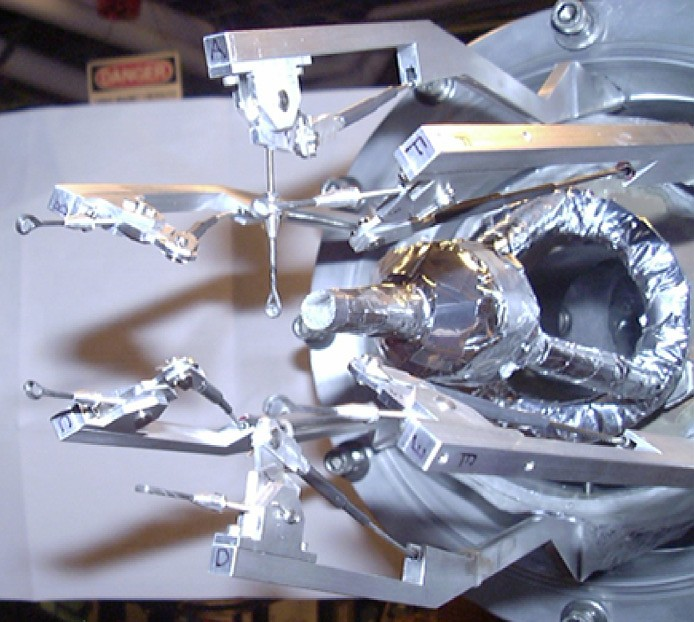
\includegraphics[width=7cm] {chap5-fig/PhTar.jpg} 
\caption {Picture of the {\it eg2} target system. The cryogenic target is 
in the back wrapped with aluminum foils, while solid targets are held by mechanical arms that were controlled remotely. In the picture, the top solid target is in the beam line.}
\label{fig:phototarget}
\end{figure}

The analysis of the experiment E-02-110, focusing on the study of color 
transparency effects, has been approved and published~\cite{ElFassi:2008}. As this 
analysis went through a careful review by the CLAS collaboration, we have adapted similar analysis methods as much as possible. In particular, the electron selection 
presented here is very similar to theirs; the main difference being a new 
target determination method. The pion identification cuts are, however, tightened
in this analysis as we have less constraints on the kinematics to exclude any possible pions' contamination.

In the section \ref{sec:pid}, we identify the following particles, e$^-$, 
$\pi^-$ and $\pi^+$ using a series of cuts on various detector outputs. For pions, we require a positive status of drift chambers (DC) and scintillator counters (SC) local signals, in addition to the global status reconstructed with the time-based tracking correction. For electron identification, we use good signals from 
all detectors, DC, Cherenkov Counters (CC), SC and the Electromagnetic 
Calorimeter (EC).

Once all particles are identified, we extract our two observables, multiplicity 
ratios and the transverse momentum broadening. Their derivation method is presented in the section \ref{sec:obs}, while a list of our corrections is summarized in the section \ref{sec:corrections}. The budget of our systematical uncertainties is detailed in the section \ref{sec:TotSys}, and the final analysis results are presented and discussed in the next chapter.

\subsection{Particle Identification}
\label{sec:pid}

\subsubsection{Electron Identification}

First, we apply a fiducial cut on the EC local coordinates to remove electrons detected close to the calorimeter's edges ($U_{EC}>40$~cm, $V_{EC}<360$~cm and 
$W_{EC}<395$~cm). These hits are problematic because part of the electromagnetic shower might be generated outside of the detector. That leads to a wrong measurement of the energy deposited.

To reject pions, we apply a momentum-dependent cut of the energy deposited in the inner ($E_{in}$) and the outer parts ($E_{out})$ of the calorimeter as,

\begin{equation}
\label{einout}
\mu  \left[1-\frac{0.3}{\sqrt{a}}\right] - \frac{E_{in}}{p} \leq 
\frac{E_{out}}{p} \leq 
\mu  \left[1+\frac{0.3}{\sqrt{b}}\right] - \frac{E_{in}}{p},
\end{equation}

where $\mu = 0.271$ is the mean of the total energy fraction deposited in the 
calorimeter, the parameter $a$ is set to 0.5, and the parameter 
$b$ varies with momenta, as shown in table \ref{tab:ecoutin-par}. The derivation of $b$ was motivated by the non-linear momentum dependence of the energy 
deposited on both EC regions (see figure \ref{eleEC}). As pions are 
minimum ionizing particles, they are expected to loose a constant energy in 
the inner part of the calorimeter (around 30~MeV), regardless of their 
momenta. Therefore, by requesting more than 60~MeV to be deposited, we 
efficiently cut the pion contamination (see figure~\ref{eleECi}).

\begin{table}[tbp]
  \centering
  \begin{tabular}{@{} cc @{}}
    \hline
    Momentum bin (GeV/c)& Parameter b \\ 
    \hline
    0.5 - 0.7 & 0.85 \\
    0.7 - 0.9 & 0.8  \\
    0.9 - 1.1 & 0.85 \\
    1.1 - 1.3 & 1.05 \\
    1.3 - 1.5 & 1.1  \\
    1.5 - 1.7 & 1.35 \\
    1.7 - 1.9 & 1.35 \\
    1.9 - 2.1 & 1.45 \\
    2.1 - 2.3 & 1.35 \\
    2.3 - 2.5 & 1.35 \\
    2.5 - 2.7 & 1.35 \\
    2.7 - 2.9 & 1.3  \\
    2.9 - 3.1 & 1.35 \\
    3.1 - 3.3 & 1.35 \\
    3.3 - 3.5 & 1.5  \\
    3.5 - 3.7 & 1.6  \\
    3.7 - 3.9 & 1.8  \\
    3.9 - 4.1 & 1.8  \\
    4.1 - 4.3 & 1.8  \\
    4.3 - 4.5 & 1.8  \\
    \hline
  \end{tabular}
  \caption{Values of the parameter $b$ used in equation \ref{einout} for 
           different momentum ranges~\cite{ElFassi:2008}.}
  \label{tab:ecoutin-par}
\end{table}

\begin{figure}[p]
\centering
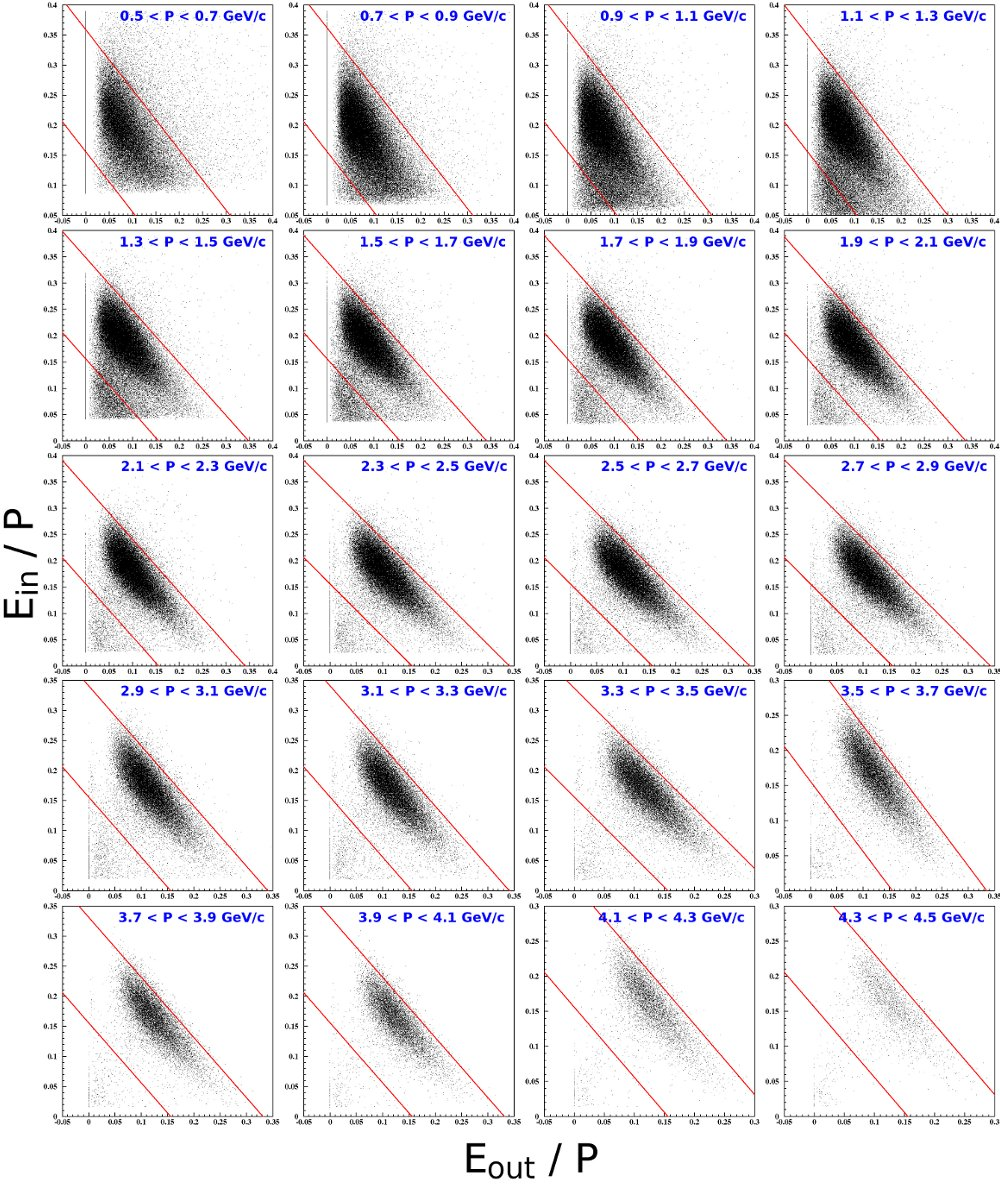
\includegraphics[width=14cm] {chap5-fig/fig02.jpg} 
\caption {Energy deposited in the inner part of the EC ($E_{in}$) as a function of the energy deposited in its outer part ($E_{out}$) normalized by tracks' momenta. Each panel is for a different momentum range, and the drawn red lines 
illustrate the cuts from equation \ref{einout}.}
\label{eleEC}
\end{figure}

\begin{figure}[tbp]
\centering
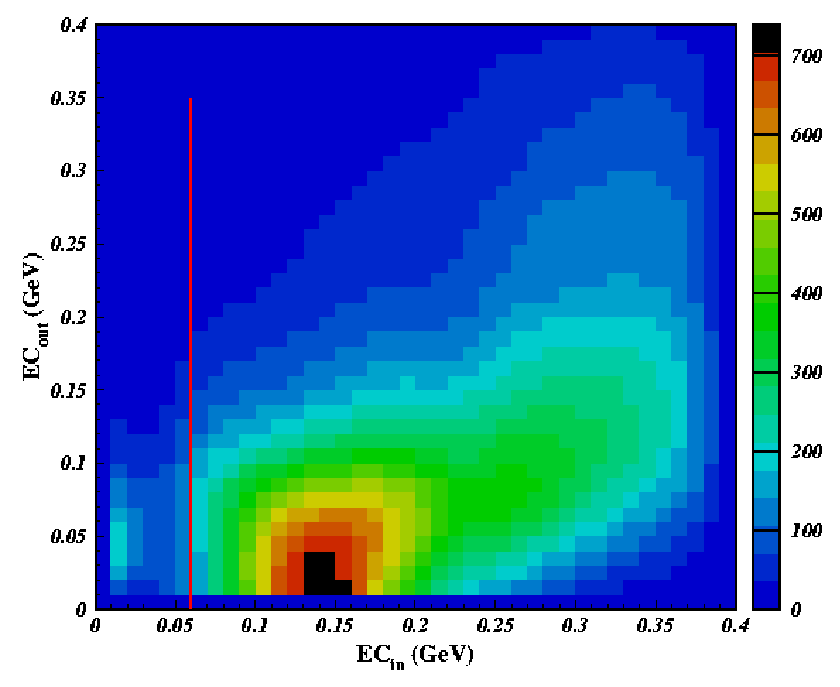
\includegraphics[width=9cm] {chap5-fig/fig03.png} 
\caption {Energy deposited in the inner part of the EC as a function of the 
energy deposited in its outer part. The red line illustrates the applied cut.}
\label{eleECi}
\end{figure}

In the CC, the mean number of photo-electrons\footnote{Photo-electrons are 
electrons produced in the front window of the Photo-Multiplier Tube (PMT) by the Cerenkov photons.} from a high energy electron is expected to be around 10.
However, hadrons can generate noise due to $\delta$ electrons produced in 
the materials of the detector. This signal is expected to be around 
one to two photo-electrons. Hence, to get rid of $\delta$-electrons, we kept only tracks with more than 2.5~photo-electrons, as depicted in figure \ref{delta}. 

\begin{figure}[tbp]
\centering
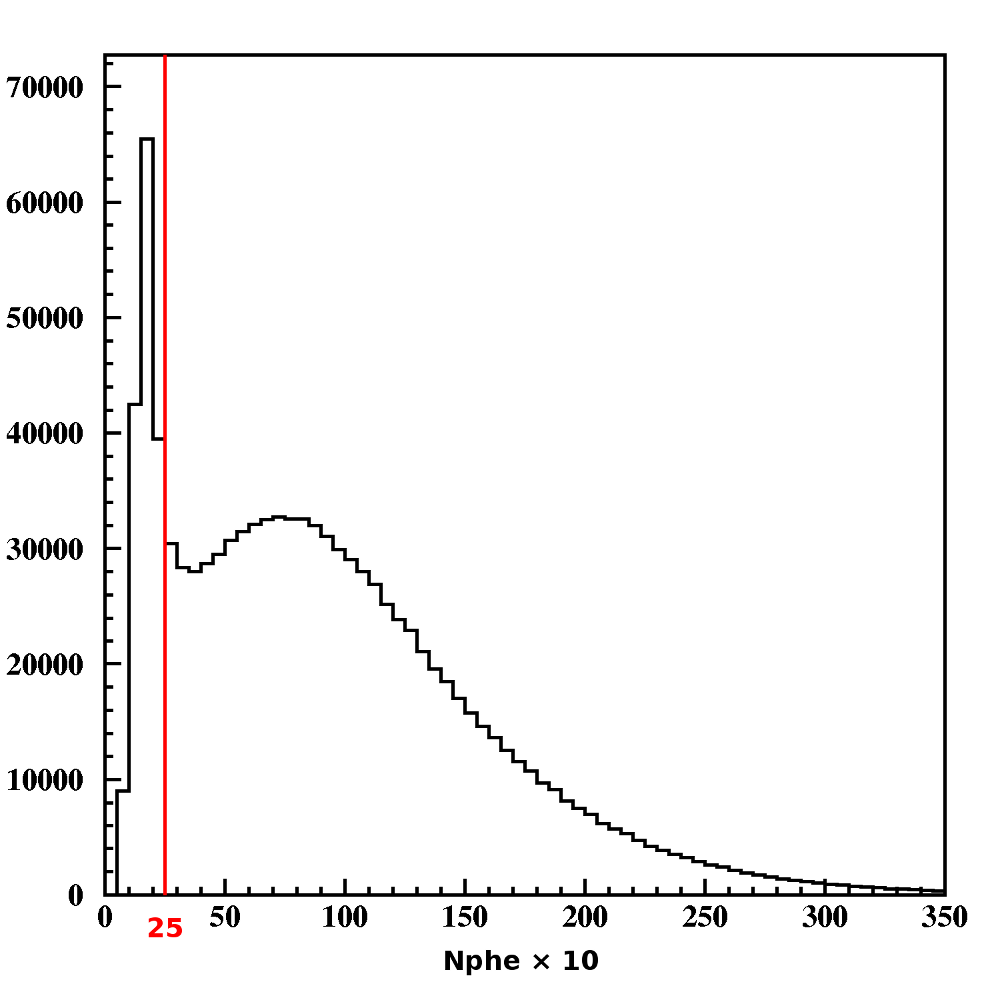
\includegraphics[width=8cm] {chap5-fig/fig04.png} 
\caption {Number of photo-electrons ($\times 10$) per tracks. The red line 
shows the applied cut to remove any low-energy pions' contamination.}
\label{delta}
\end{figure}

To select electrons, we also require that particles are negatively charged\footnote{In the CLAS reconstruction software, the electric charge is determined based on the tracks' bending direction in drift chambers.}.
Positively charged particles verifying electrons' cuts are identified as 
positrons. In the rest of this analysis, we used only events with a single electron and no positron to avoid any confusion between the scattered electron and electrons originating from hadronic decays or a photon conversion.

\subsubsection{$\pi^-$ Identification}
\label{PiId}

To identify negatively charged pions, we select negative tracks which didn't verify electrons' identification cuts. Pions are detected in the angular range from $\sim$10 to $\sim$140 degrees using only DC and SC signals.

This identification consists mostly of a time of flight (TOF) test. We define 
the relativistic particles' velocity difference as
$\Delta \beta = \beta_{measured} - {p \over \sqrt{p^2 + m_\pi^2}}$, which is required to be zero within $\pm 0.03$. Figure \ref{PionTOF} illustrates the effect of this cut. As we noticed there are not much negative kaons or anti-protons, we concluded that their contamination must be small (see section~\ref{SysId} for more detailed study).

The previous analysis from L. El Fassi et al. used $\pm 0.05$ ($\sim 3\sigma$), we decided
to reduce this number to about $2\sigma$ because of the difference of observables. The 
color transparency analysis was reconstructing the $\rho^0$ and implemented strong kinematical
cut that reduced significantly possible contaminations. Our measurement uses all the 
semi-inclusive production and is therefore more sensitive to contaminations. See next 
question for profiles.

\begin{figure}[tbp]
\centering
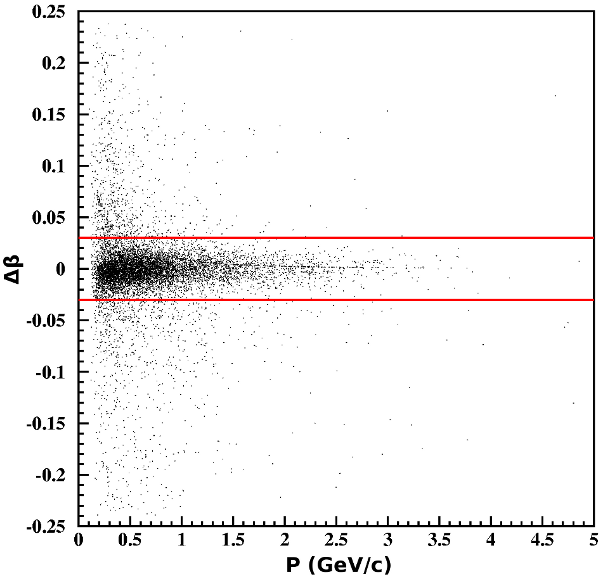
\includegraphics[width=8cm] {chap5-fig/fig05.png} 
\caption {$\Delta \beta$ of negatively charged particles as a function of momentum (GeV/c). The red lines shows the applied cuts to select negative pions.}
\label{PionTOF}
\end{figure}

In principle, a pion identification could be improved using the Cherenkov counter 
for momenta higher than 2.5~GeV/c. But, the observed low CC efficiency (see figure 
\ref{PionCC}) especially at momenta close to the CC threshold ($\sim$25\% at 
2.5~GeV/c and $\sim$50\% at 3~GeV/c) makes its use less compelling. 
Moreover, as only a very small amount of $K^-$s and no ${\bar p}s$ are present on figure \ref{PionTOF}, we decided to not use CC on this pions' identification.

\begin{figure}[tbp]
\centering
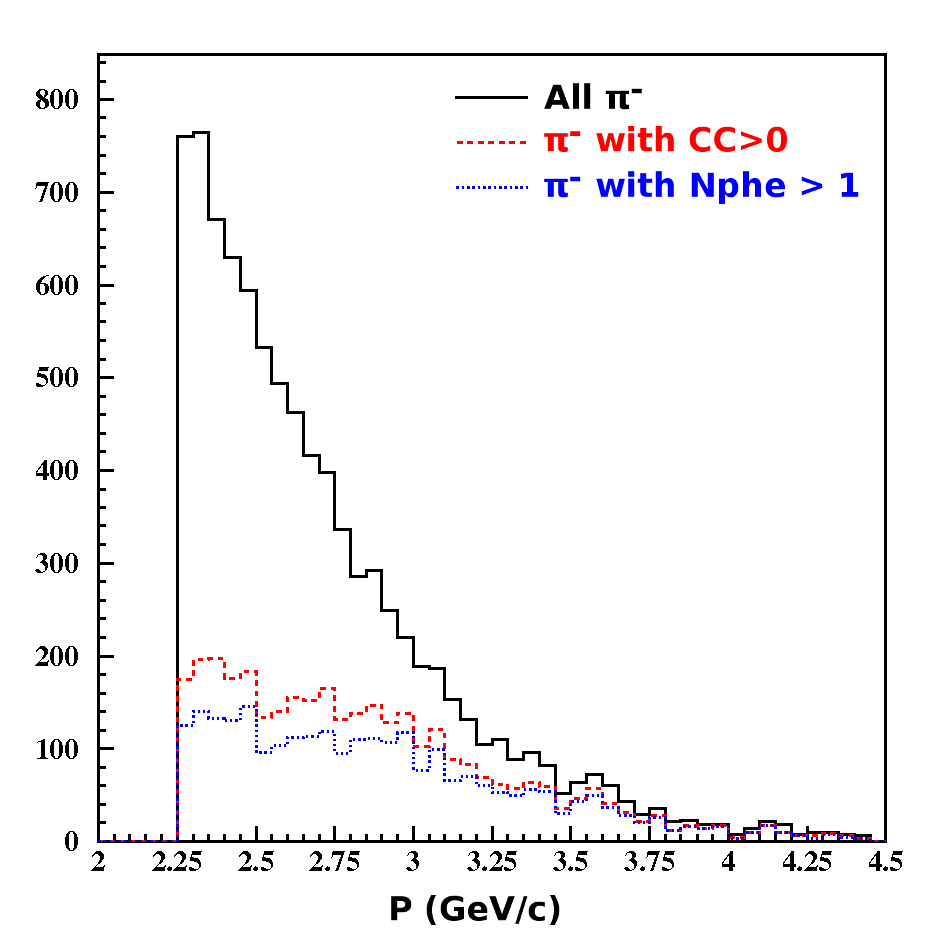
\includegraphics[width=8cm] {chap5-fig/fig06.png} 
\caption {Histograms of momentum (GeV/c) for $\pi^-$s. The black, red, and blue distributions are, respectively, for all identified $\pi^-$s, pions that fire Cherenkov counters, and pions that fire CC with more than one photo-electron.}
\label{PionCC}
\end{figure}

\subsubsection{$\pi^+$ Identification}

The identification of positively charged pions is similar to that of negative 
pions. However, the time of flight plot is significantly more busy (see figure 
\ref{PipTOF}), indicating a significant contamination from $K^+$s and protons at a
higher momentum. As the CC is not efficient enough for a hadron separation, the 
numerous kaons and protons should be removed by the following tighter TOF cuts:

\begin{subequations}\label{TOF-Pip}
\begin{align}
    p_\pi &\leq 3.375 \text{ GeV/c : }
  & \Delta \beta &> \max\left(-0.03,{p \over\sqrt{p^2+0.4^2}}\right), \\ 
    p_\pi &> 3.375    \text{ GeV/c : }
  & \Delta \beta &> \max\left(-0.02,{p \over\sqrt{p^2+0.7^2}}\right).
\end{align}
\end{subequations}

The much more apparent contamination sources than for negative pions, allow to study 
the TOF profile much more thoroughly. You can see in figures~\ref{TOF-1}, \ref{TOF-2} and 
\ref{TOF-3} the $\Delta \beta$ profiles for many momentum slices. In figure~\ref{TOF-1}
one can see some contamination from lighter leptons ($e+$ and $\mu^+$). These represent
a very small amount and one can see some justification for the choice of a $\pm 0.03$
cut as these particles do not appear to be discernable beyond that level. Similarly
in figure~\ref{TOF-2} one can see the contribution from kaons. The larger contribution
of this contamination motivated the tightening of the TOF cut on this side, to the limit
where kaons are a minority in the tail of the pion distribution. Finally a similar 
method is applied for the even larger proton contamination as shown in figure \ref{TOF-3}.

\begin{figure}[tbp]
\centering
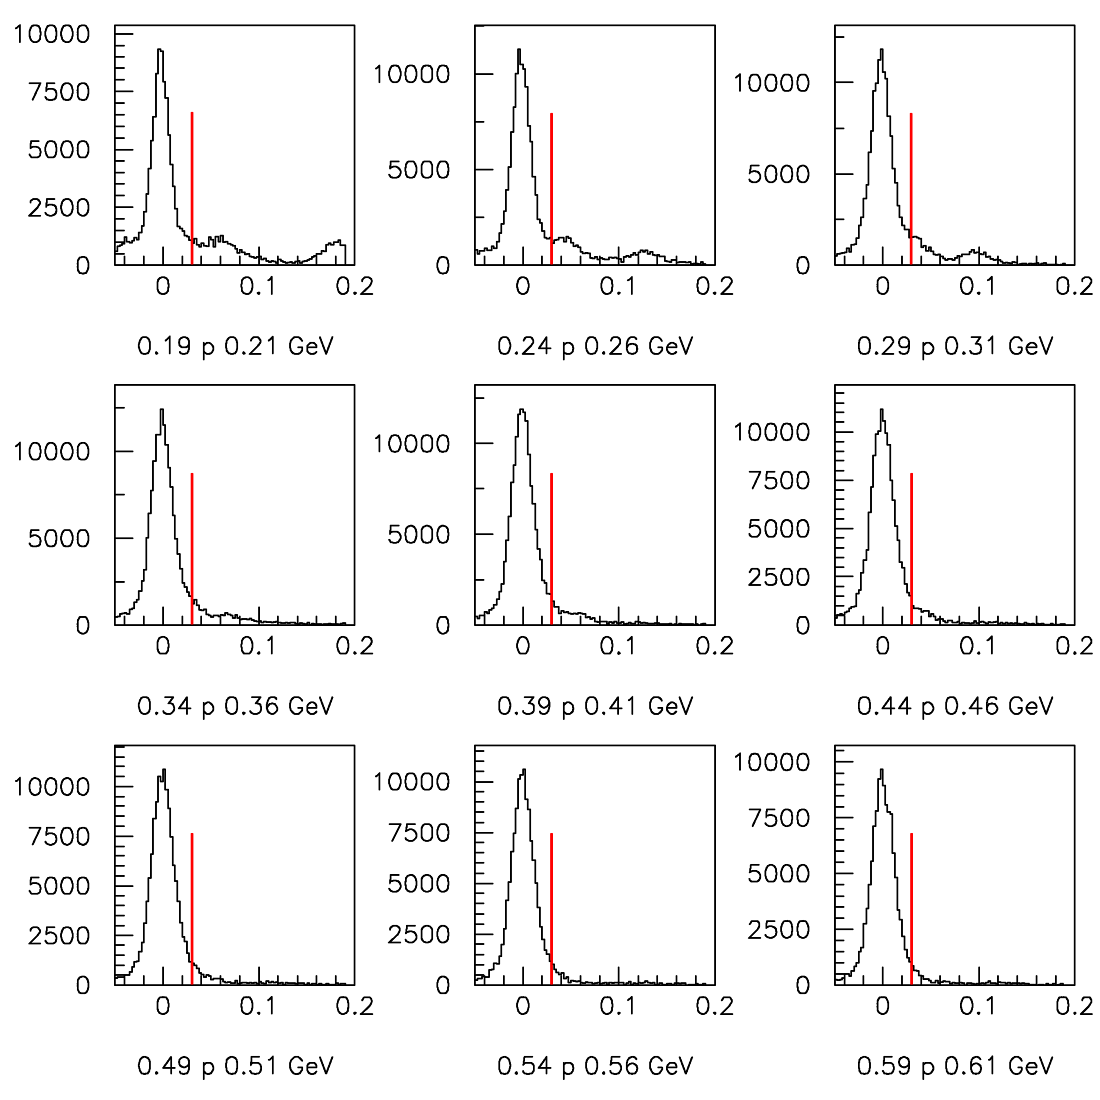
\includegraphics[width=8cm] {answer-fig/TofProfile1.png} 
\caption {$\Delta \beta$ of positively charged particles for low momentum slices 
(GeV/c). The red lines shows the applied cuts to select positive pions. The bumps on the right
correspond to muon and electron masses.}
\label{TOF-1}
\end{figure}

\begin{figure}[tbp]
\centering
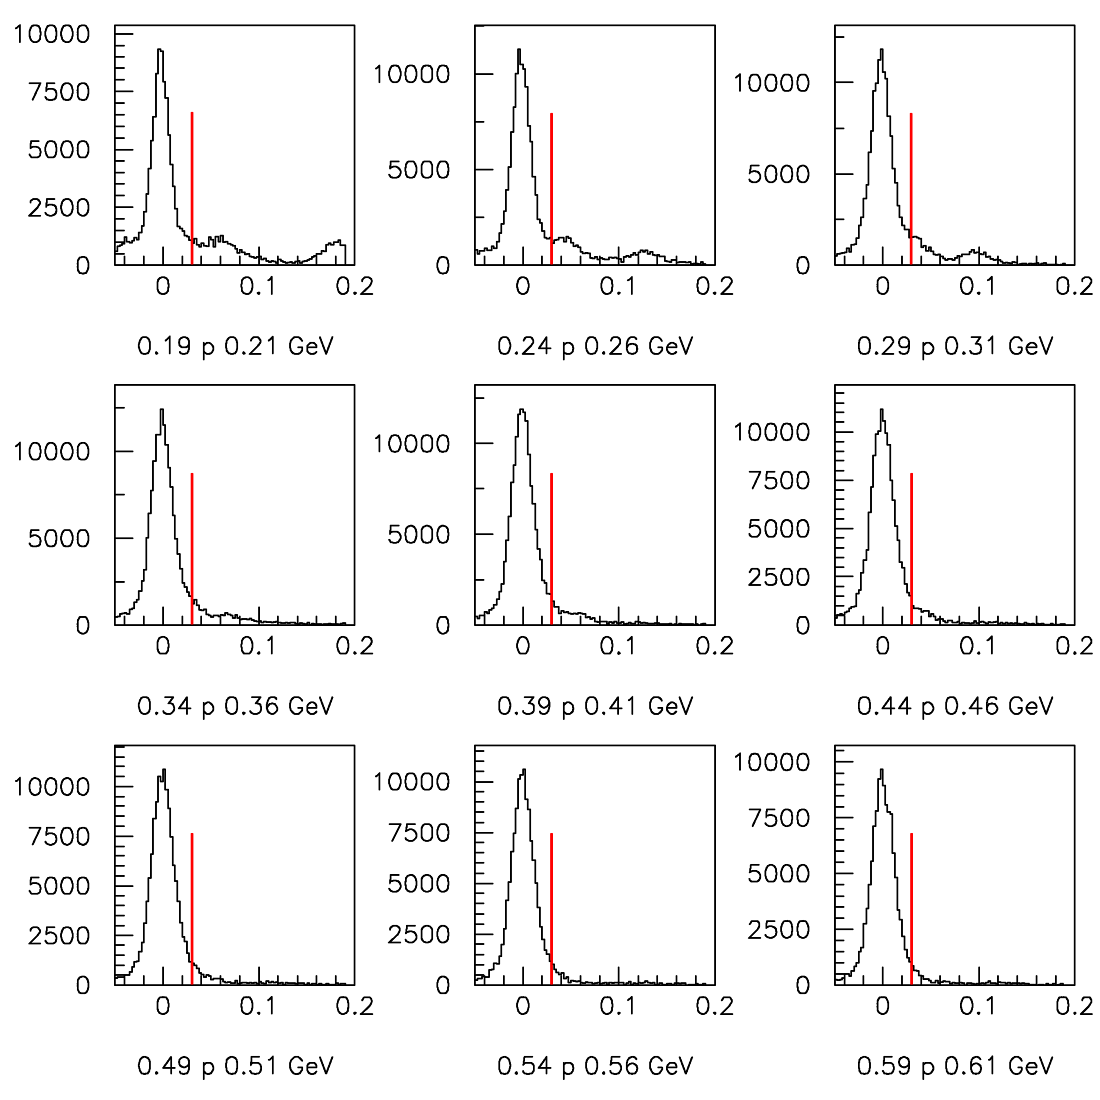
\includegraphics[width=8cm] {answer-fig/TofProfile1.png} 
\caption {$\Delta \beta$ of positively charged particles for medium momentum slices 
(GeV/c). The red lines shows the applied cuts to select positive pions. The bump on the left
correspond to the kaon mass.}
\label{TOF-2}
\end{figure}

\begin{figure}[tbp]
\centering
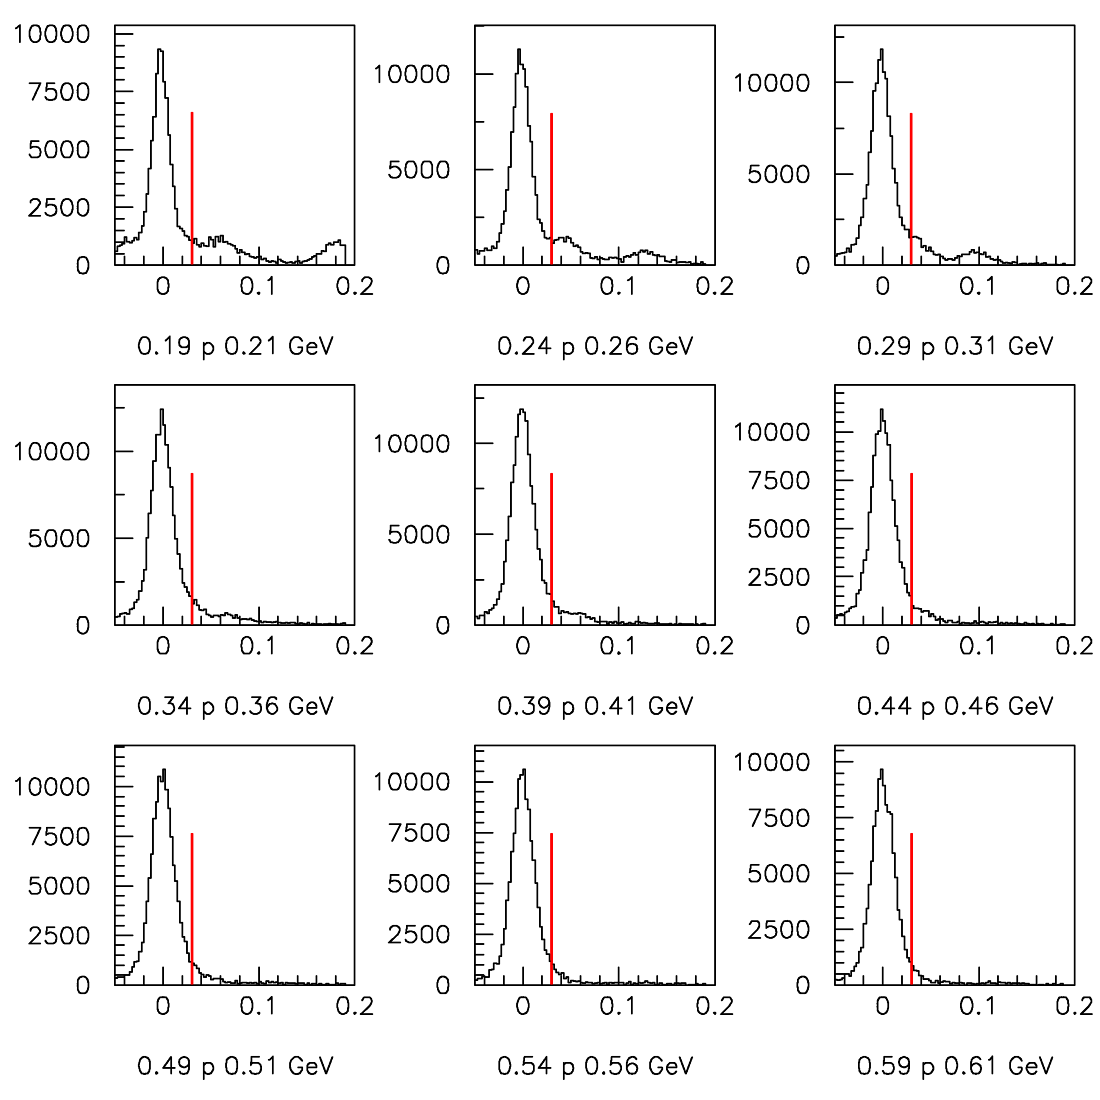
\includegraphics[width=8cm] {answer-fig/TofProfile1.png} 
\caption {$\Delta \beta$ of positively charged particles for low momentum slices 
(GeV/c). The red lines shows the applied cuts to select positive pions. The bump on the left
correspond to the proton mass.}
\label{TOF-3}
\end{figure}

These cuts permit to minimize the kaon contamination, below 2.5~GeV/c, and the 
proton contamination for all momenta. The kaon contribution cannot be avoided, however, it should remain small ($\sim$ 3\% according to simulation) 
with only a small effect on our final results (see section \ref{SysId} 
for more details). Because protons could lead to even more contamination than kaons, 
a stricter cut is used at a high momentum. This cut is also justified by 
HERMES data \cite{Airapetian:2007vu}, which showed a very different behavior of protons compared to other hadrons.

\begin{figure}[tbp]
\centering
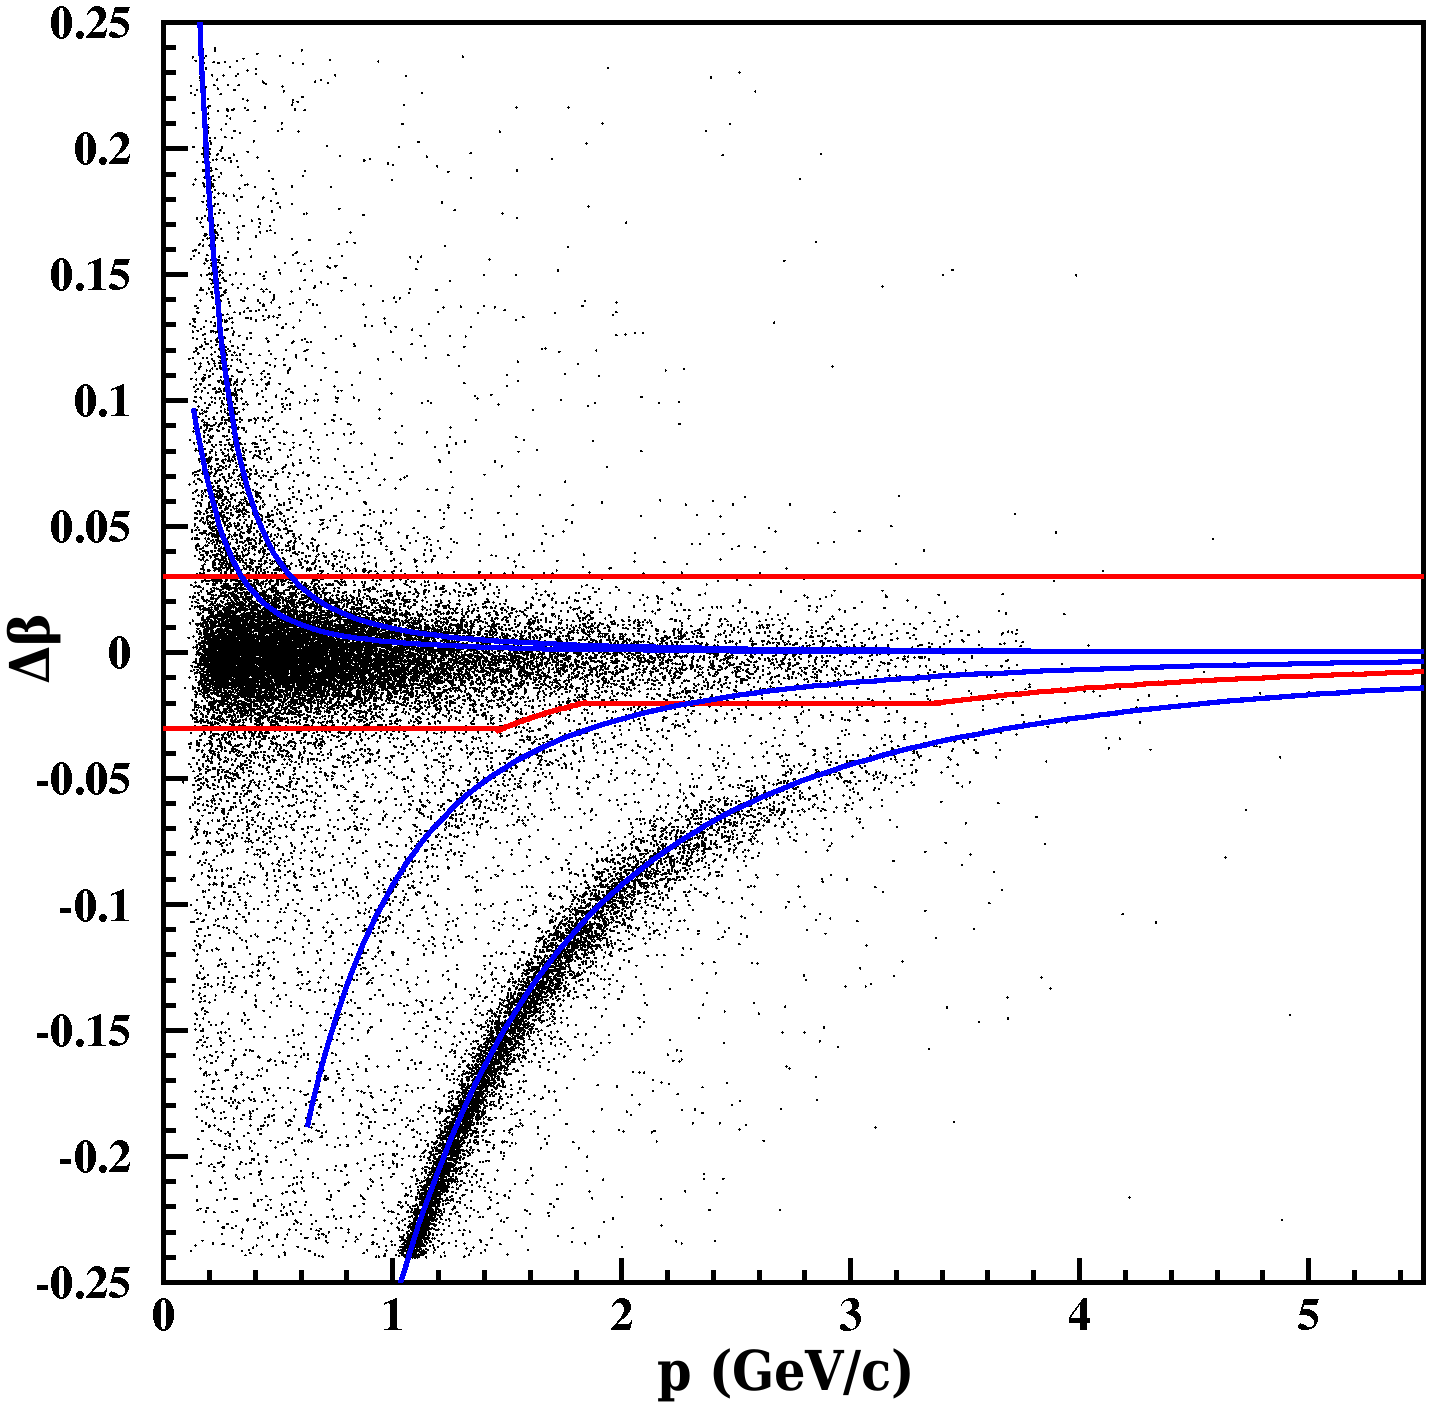
\includegraphics[width=8cm] {chap5-fig/pip_data.png} 
\caption {$\Delta \beta$ of positively charged particles as a function of momentum (GeV/c). The red lines shows the applied cuts to select positive pions. The blue lines indicate other particles' theoretical positions, and present from top to 
bottom positrons, muons, kaons and protons.}
\label{PipTOF}
\end{figure}

\subsubsection{Target Determination}

To differentiate between the two targets and remove the background, we need to 
determine the origin of our final-state particles. As illustrated in figure~\ref{vertex}, the small misalignment of the beam with the CLAS detector led to an artificial shift on different sectors' z-vertex positions. To correct from this effect, we added the shift shown in table~\ref{tab:vertex} when determining each particle's vertex position. Those values were obtained from the fit of the solid target distribution on each sector.

\begin{table}[p]
  \centering
  \begin{tabular}{@{} cc @{}}
    \hline
    Sector & Shift (cm) \\ 
    \hline
    1 & + 0.1 \\ 
    2 & - 0.4 \\ 
    3 & - 0.6 \\ 
    4 & - 0.1 \\ 
    5 & + 0.4 \\ 
    6 & + 0.6 \\ 
    \hline
  \end{tabular}
  \caption{Values used to correct the vertex position on each sector}
  \label{tab:vertex}
\end{table}

The position of our targets could also vary from a run to another, but this was not significant in this experiment. Indeed, except for aluminum, other targets remained in the same position within one or two millimeters. All targets' positions, in CLAS coordinates, are given in table \ref{tab:targets}. 
We show in figures \ref{VertexSolid} and \ref{VertexLiquid} the evolution 
of the position of the targets with run number. The data where the aluminum
target is off by 1 cm has been excluded from the analysis. Other variations
appear to be of a mm or less, while the gap between the solid and liquid target
is about 5 cm. They should therefore have negligible contribution to the 
error on acceptance corrections in regard to the error budget already associated
to the procedure.

\begin{table}[p]
  \centering
  \begin{tabular}{|c|c|c|c|c|c|c|}
    \hline
    Target & Carbon & Al (1) & Al (2) & Iron   & Tin    & Lead   \\ 
    \hline \hline
    Liquid & -30.1  & n/a    & n/a    & -30.2  & -30.1  & -30.1  \\ 
    Solid  & -24.7  & -25.0  & -23.8  & -24.9  & -23.8  & -24.9  \\
    \hline
  \end{tabular}
  \caption{The measured mean vertex position of our nuclear targets relative to the center of CLAS (in cm). Must note that aluminum data are separated in two sets because this target's position has brutally changed. Moreover, during these runs the deuterium target was empty.}
  \label{tab:targets}
\end{table}

\begin{figure}[tbp]
\centering
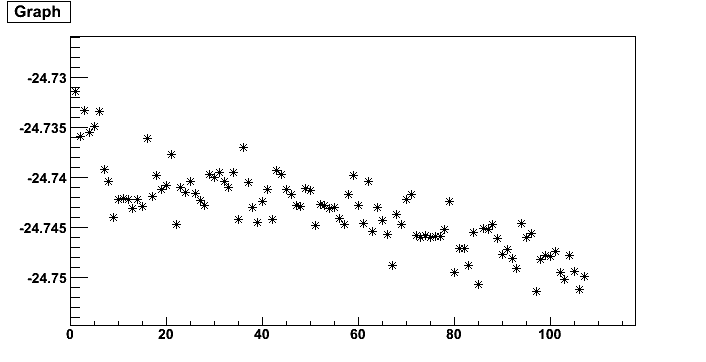
\includegraphics[width=7.5cm] {answer-fig/VertexC.png} 
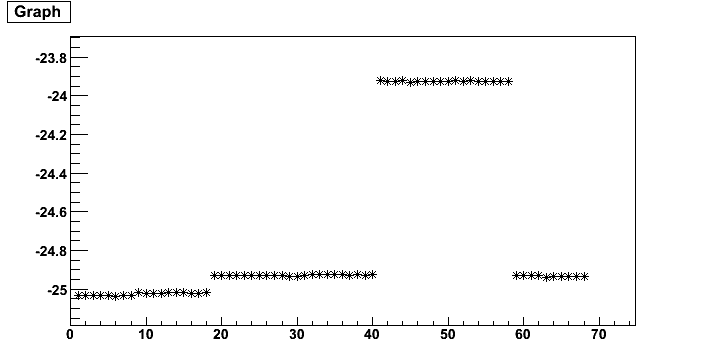
\includegraphics[width=7.5cm] {answer-fig/VertexAl.png} 
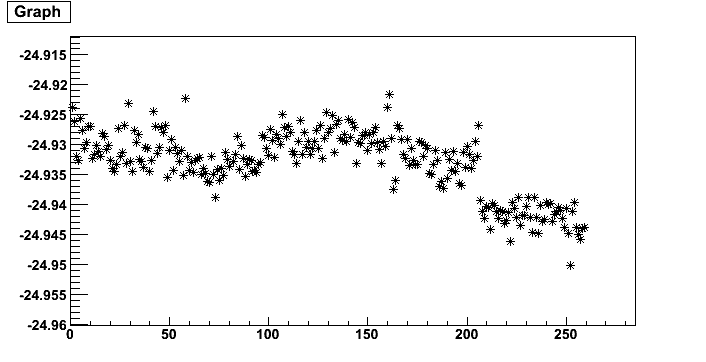
\includegraphics[width=7.5cm] {answer-fig/VertexFe.png} 
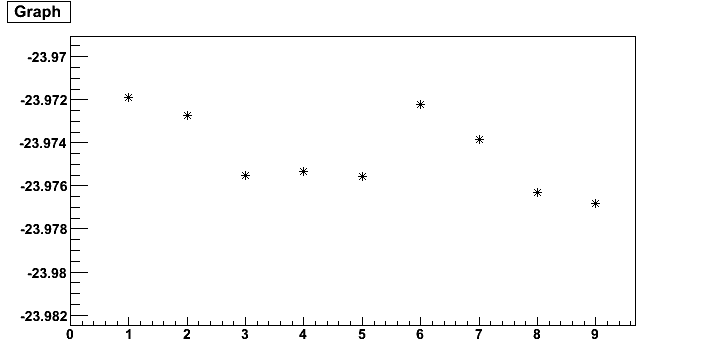
\includegraphics[width=7.5cm] {answer-fig/VertexSn.png} 
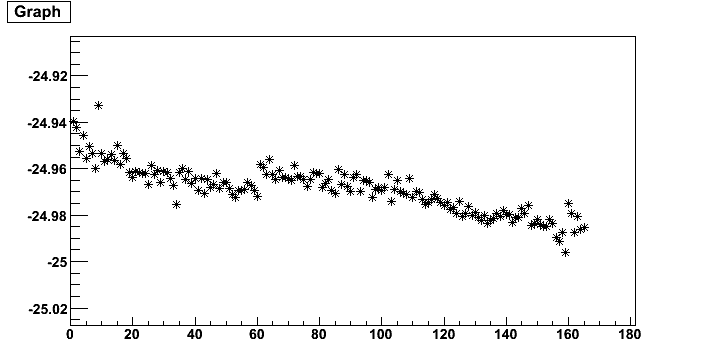
\includegraphics[width=7.5cm] {answer-fig/VertexPb.png} 
\caption {Vertex origin along $z$ (in cm) of electrons as a function of run 
number for the different solid targets.}
\label{VertexSolid}
\end{figure}

\begin{figure}[tbp]
\centering
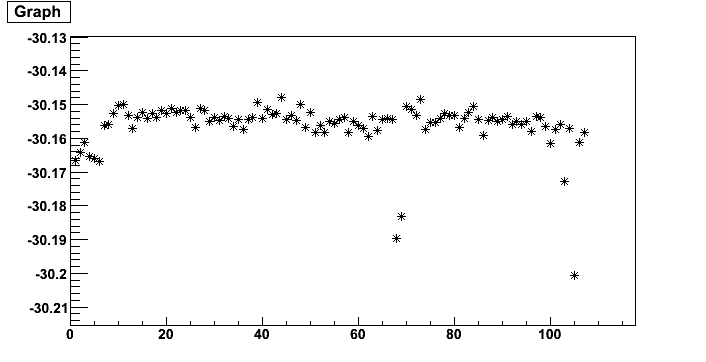
\includegraphics[width=7.5cm] {answer-fig/VertexDeutC.png} 
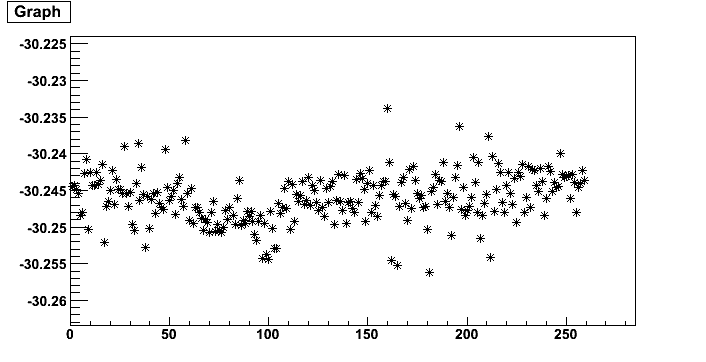
\includegraphics[width=7.5cm] {answer-fig/VertexDeutFe.png} 
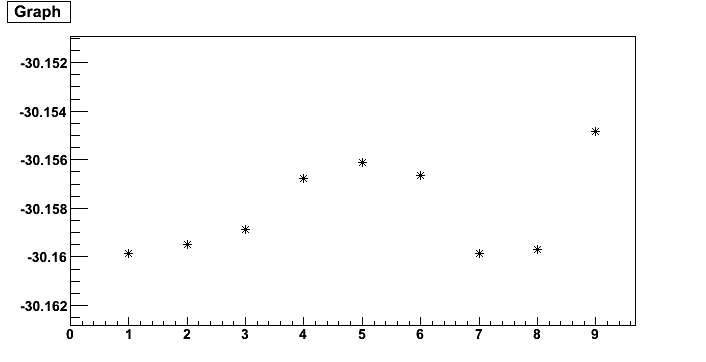
\includegraphics[width=7.5cm] {answer-fig/VertexDeutSn.png} 
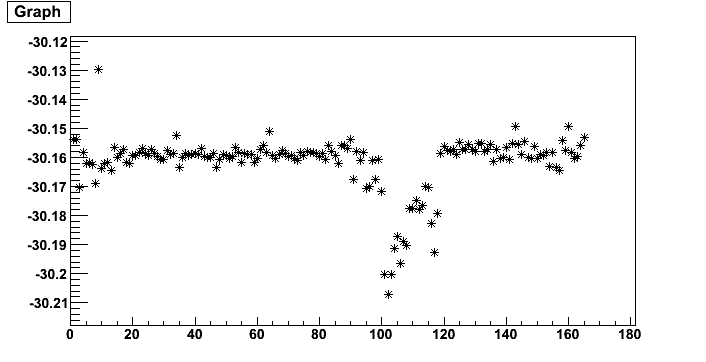
\includegraphics[width=7.5cm] {answer-fig/VertexDeutPb.png} 
\caption {Vertex origin along $z$ (in cm) of electrons as a function of run 
number for the deuterium target in different solid targets configurations.}
\label{VertexLiquid}
\end{figure}

The detected electrons are associated with the solid target if their vertex 
position is less than 1.5~cm ($\sim$3~$\sigma$) from the values shown on table 
\ref{tab:targets}. For the liquid target, the cut is a bit larger, 2 cm, in order to count for the cryogenic target's size (see figure \ref{vertex}). The pions' vertex was checked against the electron one and was imposed to satisfy this additional condition $| Vz^{e^-} - Vz^{\pi} | < 3$ cm (see figure \ref{fig:dvzpi}).

\begin{figure}[p]
\centering
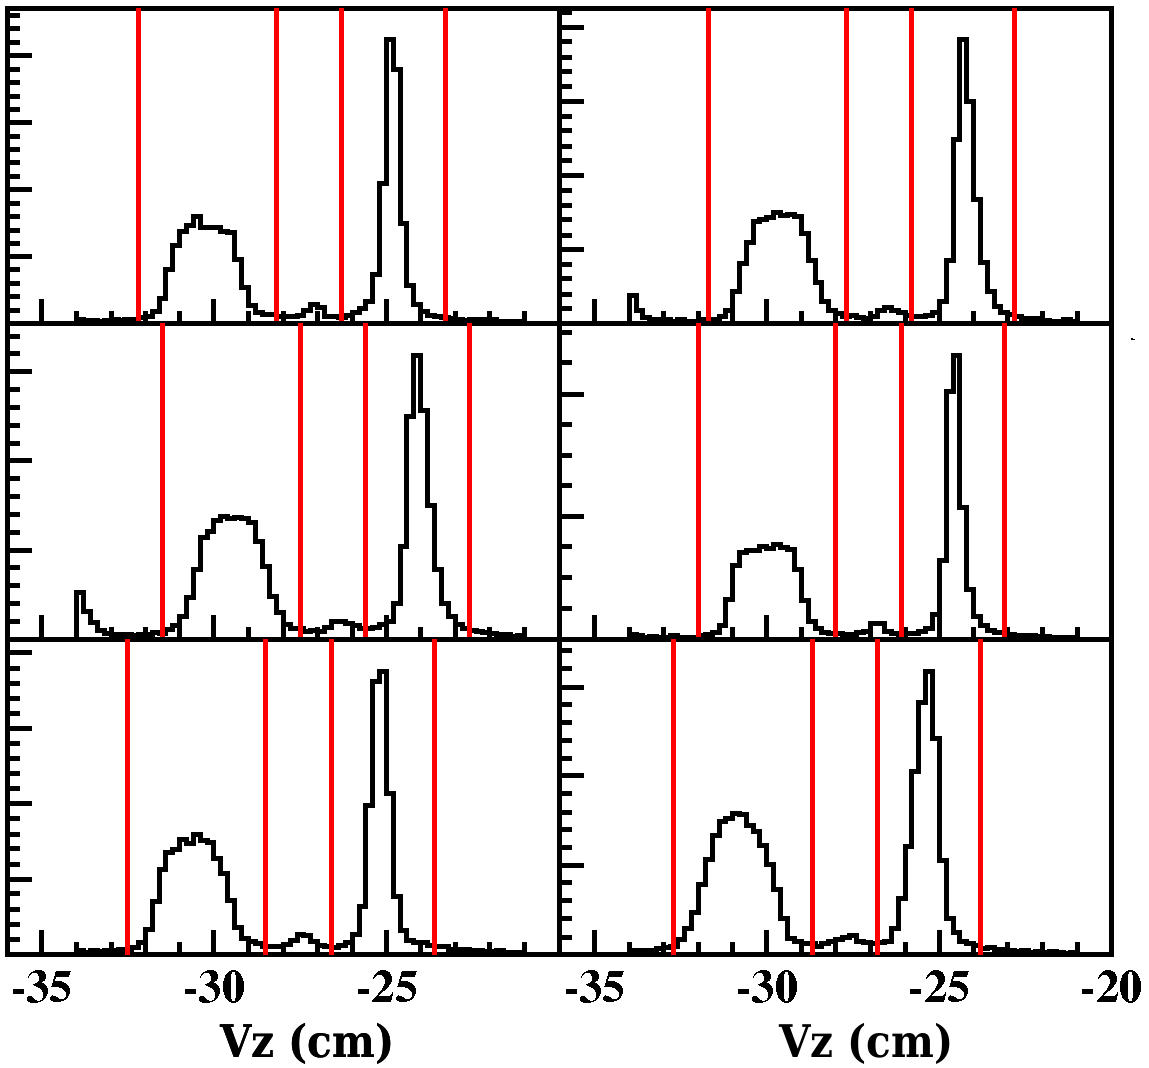
\includegraphics[width=10cm] {chap5-fig/Vertex_el_data.png}
\caption {Sector-by-sector electrons' vertex distributions. The latter are reconstructed along the beam direction and relative to the center of CLAS located at 0~cm. The red lines show the applied cuts to select the two targets.}
\label{vertex}
\end{figure}

\begin{figure}[tbp]
\centering
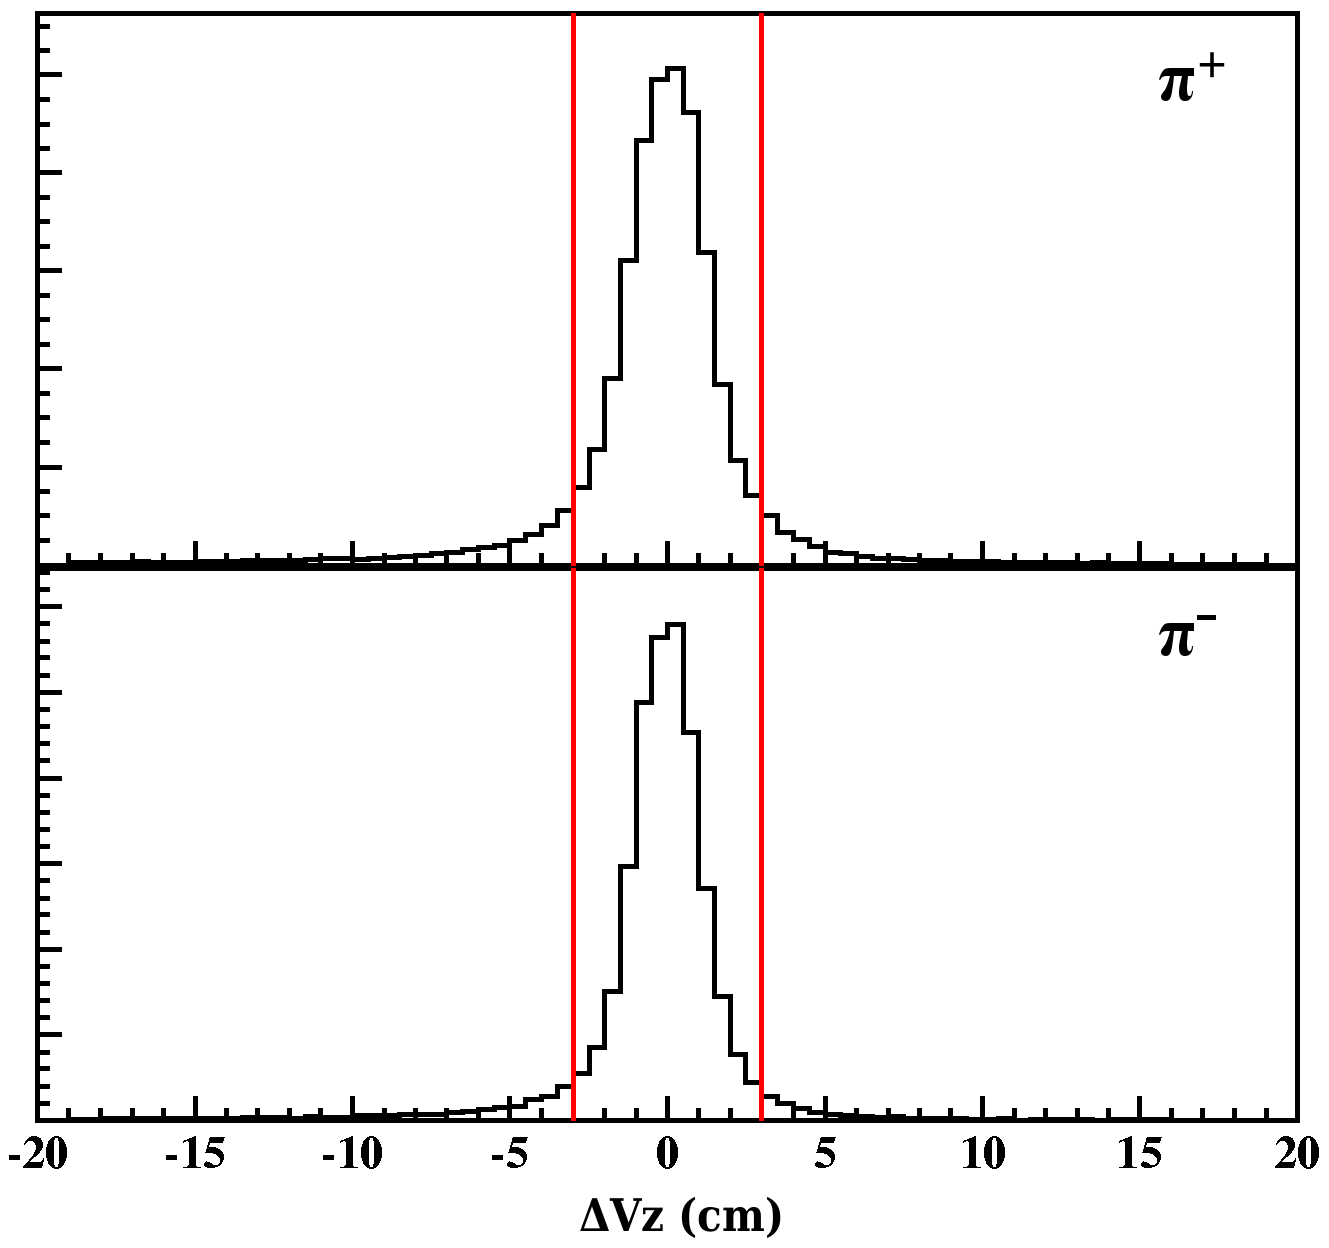
\includegraphics[width=8cm] {chap5-fig/Vertex_pi_data.png}
\caption {The difference between electrons and pions z-vertex positions. $\pi^+$s and $\pi^-$ are plotted, respectively, in the top and bottom panels. The red lines show the applied cuts to select both pions.}
\label{fig:dvzpi}
\end{figure}

\subsubsection{Data Quality}

To check the quality of the runs\footnote{Runs were formed roughly from two hours
of data, but they were much smaller in case of problems.}, we monitored the ratio of scattered electrons yields obtained from solid and liquid targets. In case of the beam hitting other materials in the beam-line or of ony other problem that would affect our final result, 
this ratio will be off and indicate the problematic runs. A figure 
\ref{DataQ} shows electrons yields' ratios for different nuclear target; we fitted these ratios to extract the mean value for each target, then we discarded runs that were 5~$\sigma$ away from the appropriate mean. Must note that these ratios were consistent with our target's thicknesses given in \cite{Hakobyan:2008zz} except for a carbon target. For that reason, the density of the latter was recently remeasured, and its new value was finally matching our data\footnote{i.e. (1.747+/-0.0007)g/cm$^3$ instead of 2.235 g/cm$^3$}.

\begin{figure}[tbp]
\centering
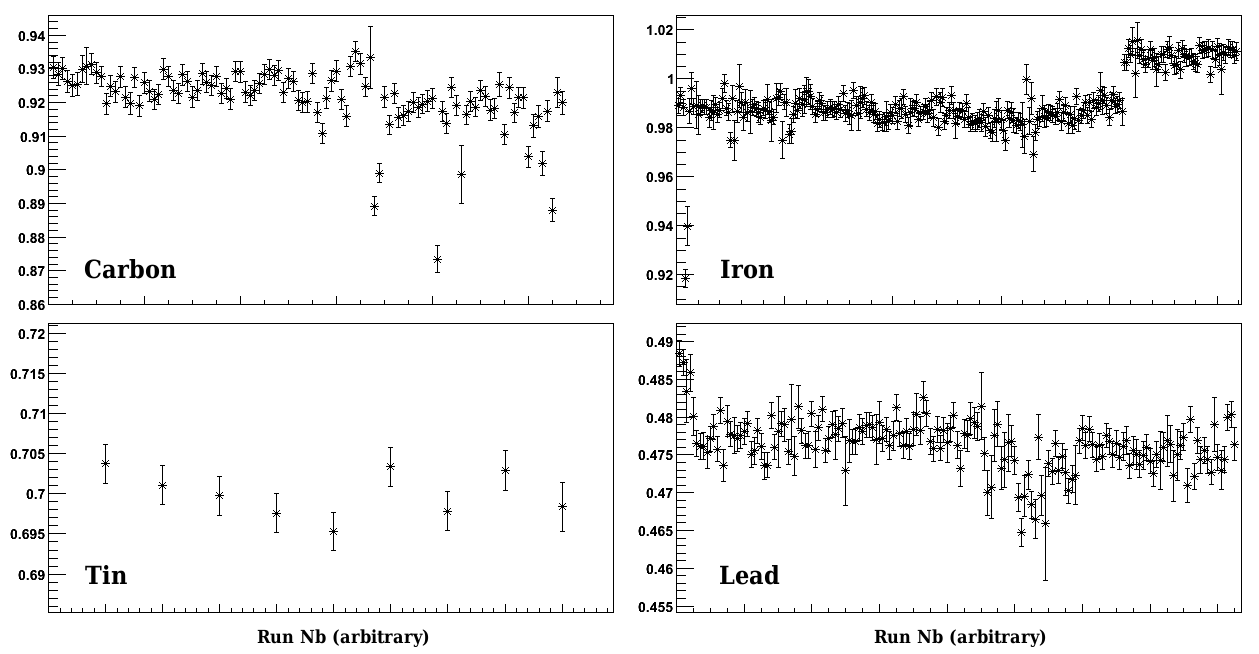
\includegraphics[width=15cm] {chap5-fig/TargetElRatio.png}
\caption {Ratio of scattered electrons yields (solid over deuterium) for each run.}
\label{DataQ}
\end{figure}

\subsection{Extraction of Multiplicity Ratio and $\Delta$P$_\perp^2$}
\label{sec:obs}

Since we are interested in deep inelastic scattering, we use the following 
cuts: $Q^2 > 1$~GeV$^2$/c$^2$ and $W > 2$~GeV/c$^2$, with the inclusive distributions
after these cuts shown in figure \ref{DISKine}.

\begin{figure}[tbp]
\centering
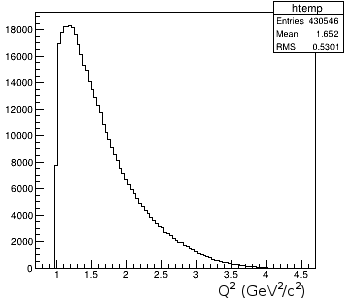
\includegraphics[width=5cm] {answer-fig/DIS-Q2.png} 
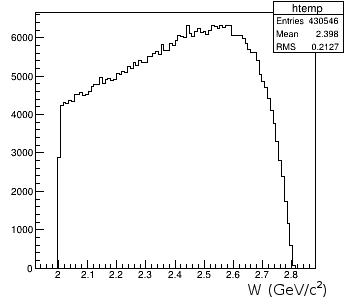
\includegraphics[width=5cm] {answer-fig/DIS-w.png} 
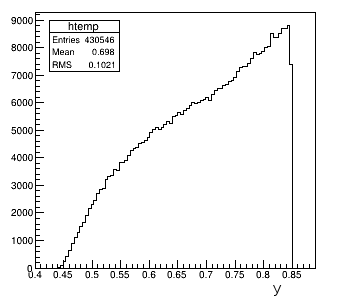
\includegraphics[width=5cm] {answer-fig/DIS-y.png} 
\caption {Inclusive distributions after DIS selection cuts for a sample of the iron
data.}
\label{DISKine}
\end{figure}

We also apply a cut on the energy transferred fraction, $y = \nu/E_{beam} < 0.85$. This cut aims to remove the low energy electrons that are significantly affected by radiative effects and sat at the limit of our trigger threshold.

\subsubsection{Method}
\label{RatioCalc}

Once the identification is done, the calculation of our two observables and their statistical uncertainties is straightforward. The latter are given by:
\begin{equation}
{\delta \left ( R_A^h \right ) \over R_A^h} = \sqrt{ 1 /N_A^h + 1/ N_A^e +1/N_D^h + 1/N_D^e}
\end{equation}
and
\begin{equation}
\left ( \delta \left ( \Delta \langle P_\perp^2 \rangle \right ) \right )^2 = 
   \left ({\langle P_\perp^4 \rangle - \langle P_\perp^2 \rangle ^2}\right )_A / N_A^h
 + \left ({\langle P_\perp^4 \rangle - \langle P_\perp^2 \rangle ^2}\right )_D / N_D^h.
\end{equation}

However, the implementation of acceptance and radiative corrections is done through some given weights to each event based on its kinematics. The multiplicity ratio then becomes
\begin{equation}
R_A^h (Q^2,\nu,z_h,P_\perp^2) = {{\sum \omega_A^h (Q^2,\nu,z_h,P_\perp^2) / \sum \omega_A^e (Q^2,\nu)} 
                       \over {\sum \omega_D^h (Q^2,\nu,z_h,P_\perp^2) / \sum \omega_D^e (Q^2,\nu)}},
\end{equation}
where $\omega$ is the weight associated with the event, and the sums run over all measured particles. The expression of the transverse momentum broadening remains as
\begin{equation}
\Delta \langle P_\perp^2 \rangle = \langle P_\perp^2 \rangle_A - \langle P_\perp^2 \rangle_D,
\end{equation}
but with
\begin{equation}
\langle P_\perp^2 \rangle = {\sum \left ( P_\perp^2 \times \omega (Q^2,\nu,z_h,P_\perp^2) \right ) \over \sum \omega (Q^2,\nu,z_h,P_\perp^2)}.
\end{equation}

Thus, new expressions of the weighted statistical uncertainties are: 
\begin{equation}
{\delta \left ( R_A^h \right ) \over R_A^h} = 
      \sqrt{ \left ( {\sum {\omega^h_A}^2 \over \left (\sum \omega^h_A \right )^2} \right ) 
           + \left ( {\sum {\omega^e_A}^2 \over \left (\sum \omega^e_A \right )^2} \right ) 
           + \left ( {\sum {\omega^h_D}^2 \over \left (\sum \omega^h_D \right )^2} \right ) 
           + \left ( {\sum {\omega^e_D}^2 \over \left (\sum \omega^e_D \right )^2} \right ) }
\end{equation}
 and 
\begin{equation}
\begin{split}
\left ( \delta \left ( \Delta \langle P_\perp^2 \rangle \right ) \right )^2 = 
   \left ({{\sum \omega^h_A P_\perp^4 }\over{\sum \omega^h_A}} - \left ({\sum \omega^h_A P_\perp^2 }\over{\sum \omega^h_A}\right )^2 \right ) 
         \times \left ( {\sum \left ( {\omega^h_A}^2 \right ) \over \left ( \sum \omega^h_A \right ) ^2 }\right ) \\
 + \left ({{\sum \omega^h_D P_\perp^4 }\over{\sum \omega^h_D}} - \left ({\sum \omega^h_D P_\perp^2 }\over{\sum \omega^h_D}\right )^2 \right ) 
	 \times \left ( {\sum \left ( {\omega^h_D}^2 \right ) \over \left ( \sum \omega^h_D \right ) ^2 }\right ).
\end{split}
\end{equation}

\subsubsection{Preliminary Results}
\label{prelim}

To provide some insight into the quality of our data, we present in figure~\ref{fig:prelim} few preliminary results before the application of any corrections. These preliminary results will be used also to illustrate the effects of the corrections discussed below.

\begin{figure}[htb]
\centering
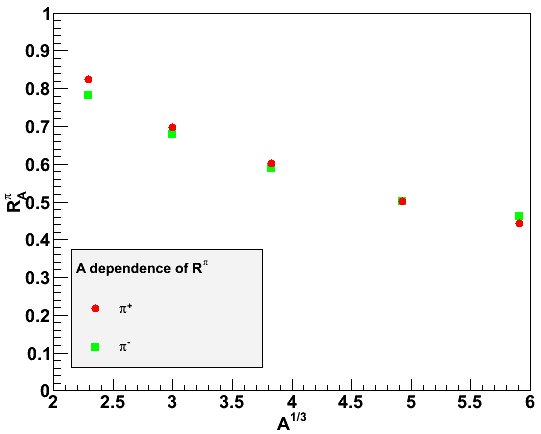
\includegraphics[width=7.4cm] {chap5-fig/a_RvA.png} 
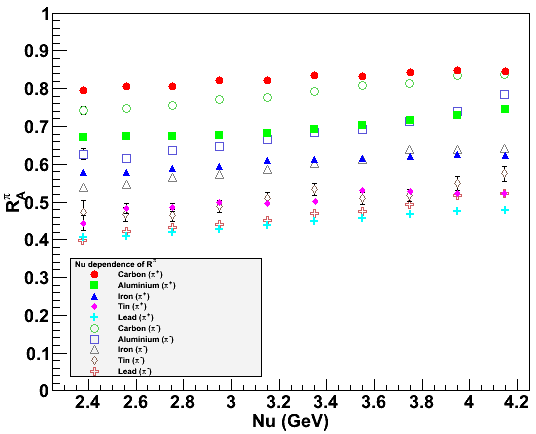
\includegraphics[width=7.4cm] {chap5-fig/a_RvZ.png} 
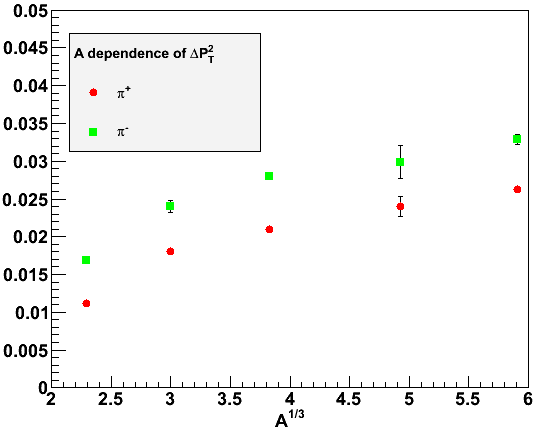
\includegraphics[width=7.4cm] {chap5-fig/a_PvA.png} 
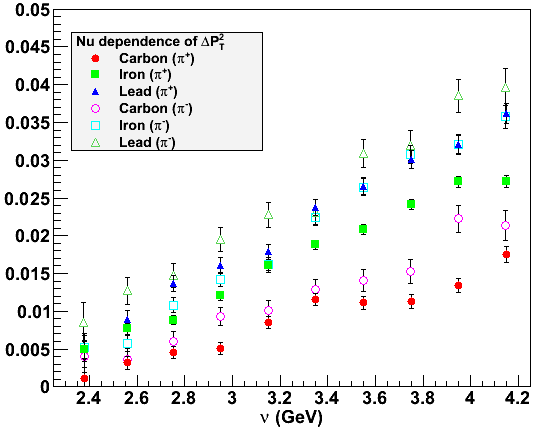
\includegraphics[width=7.4cm] {chap5-fig/a_PvNu.png} 
\caption {Results for multiplicity ratios (top) and the transverse momentum 
broadening (bottom) before applying any corrections.}
\label{fig:prelim}
\end{figure}


\subsection{Corrections}
\label{sec:corrections}

\subsubsection{Acceptance Correction}
\label{sec:accept}

The acceptance correction consists of applying weights to the experimental data
event by event to correct for any detection inefficiencies of used detectors.
Incidentally, it also corrects for other small detection issues, such as misidentification and re-scattering on detectors' materials. The quality 
of the correction depends on the ability of the simulation to reproduce the 
experiment, the accumulated statistics, and the size of interfering effects, such 
as the bin migration. For this correction, we applied the method from the 
approved and published analysis from the same eg2 data~\cite{ElFassi:2008}.

\paragraph{Simulation}
\label{sec:simul}

To correct for acceptance effects, we simulated a total of 100 million events 
per target ($^2$H, C, Fe and Pb) using the PYTHIA \cite{Sjostrand:2006za} 
event generator that was slightly modified to include Fermi motion effects. The 
generated events are processed by CLAS softwares (GSIM, GPP and user\_ana) 
to simulate the detector and the reconstruction process similarly to the experimental data.
% TODO GPP factors

Then the simulated data are processed in a similar way than the experimental data by 
applying the cuts described in the section \ref{sec:pid}. Overall the 
simulation reproduces quite well the detectors responses, yet two issues might 
affect us and have to be understood. First, the efficiency of the CC is 
overestimated in the simulation. On the electron side the signal is a little stronger in the simulation (11 
photo-electrons) compared to experimental data (8 photo-electrons), but this 
feature should not affect us too much, because we are cutting only the tail of the 
distribution in both cases. Second, since in the simulation the beam is perfectly aligned with CLAS, the vertex cuts do not need to be shifted from one sector to an other. Therefore, we do not apply the shift from table \ref{tab:vertex} to the simulated data; the resulting cuts are shown in figure~\ref{simvertex}.

\begin{figure}[tpb]
\centering
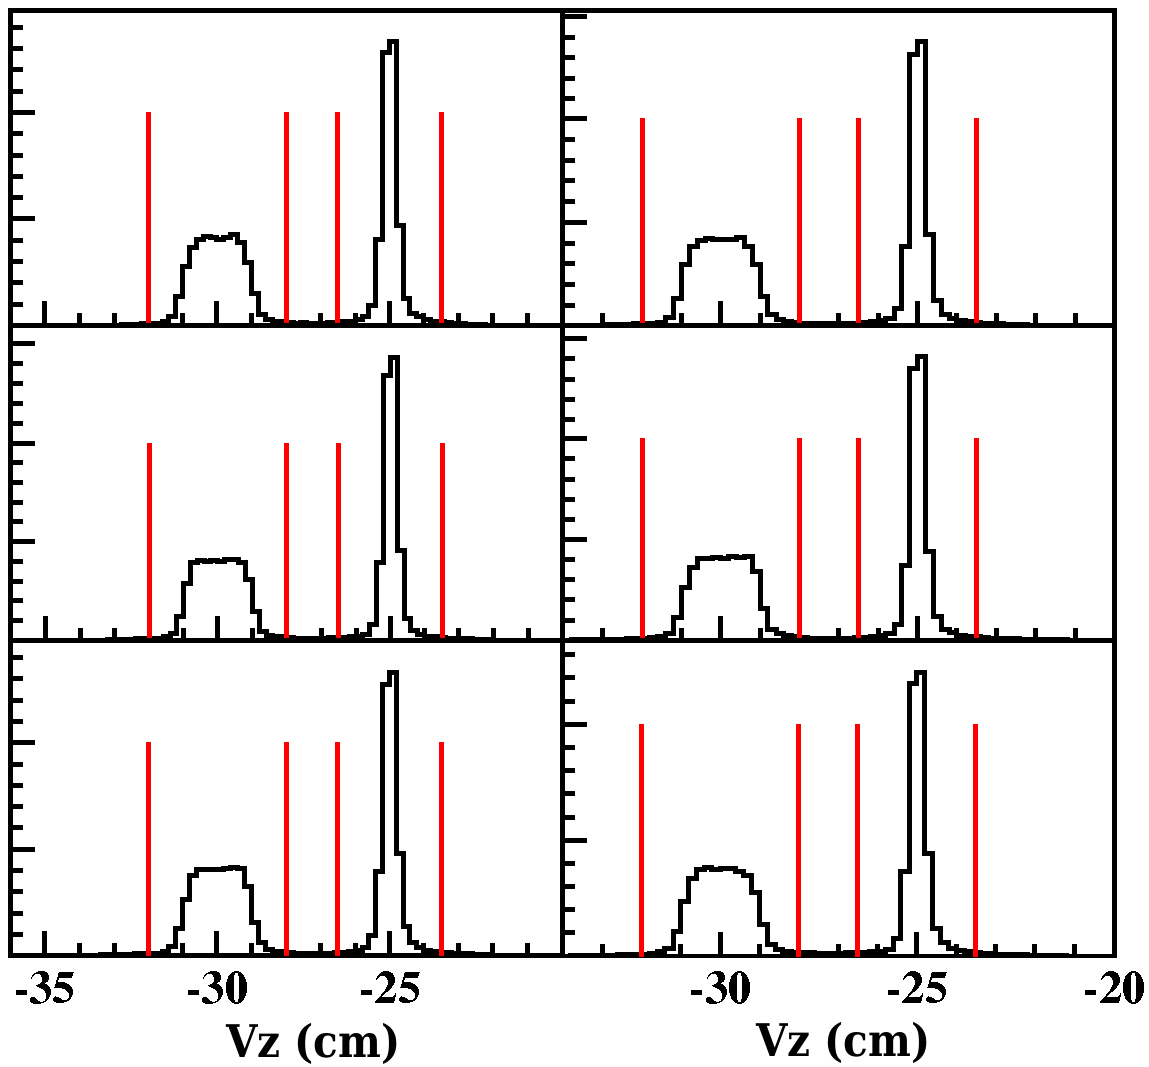
\includegraphics[width=9cm] {chap5-fig/Vertex_el_sim.png}
\caption {Sector by sector electrons' vertex distributions from the {\bf simulated data}. The latter are reconstructed along the beam direction, and relative to the CLAS center. The red lines show the used cuts to select both targets.}
\label{simvertex}
\end{figure}

The kinematical distributions from the simulation are compared to the 
experimental ones. This is important for the acceptance correction, to see 
whether or not, we can integrate over any variables in this correction.
Comparisons between simulated and experimental data are shown in figures 
\ref{fig:compNuQ2} to \ref{fig:compPhih}. The agreement is reasonable, but not 
perfect. The differences are due to the PYTHIA simulation, which is not including some 
physical effects, such as radiative and diffractive processes.

\begin{figure}[tbp]
\centering
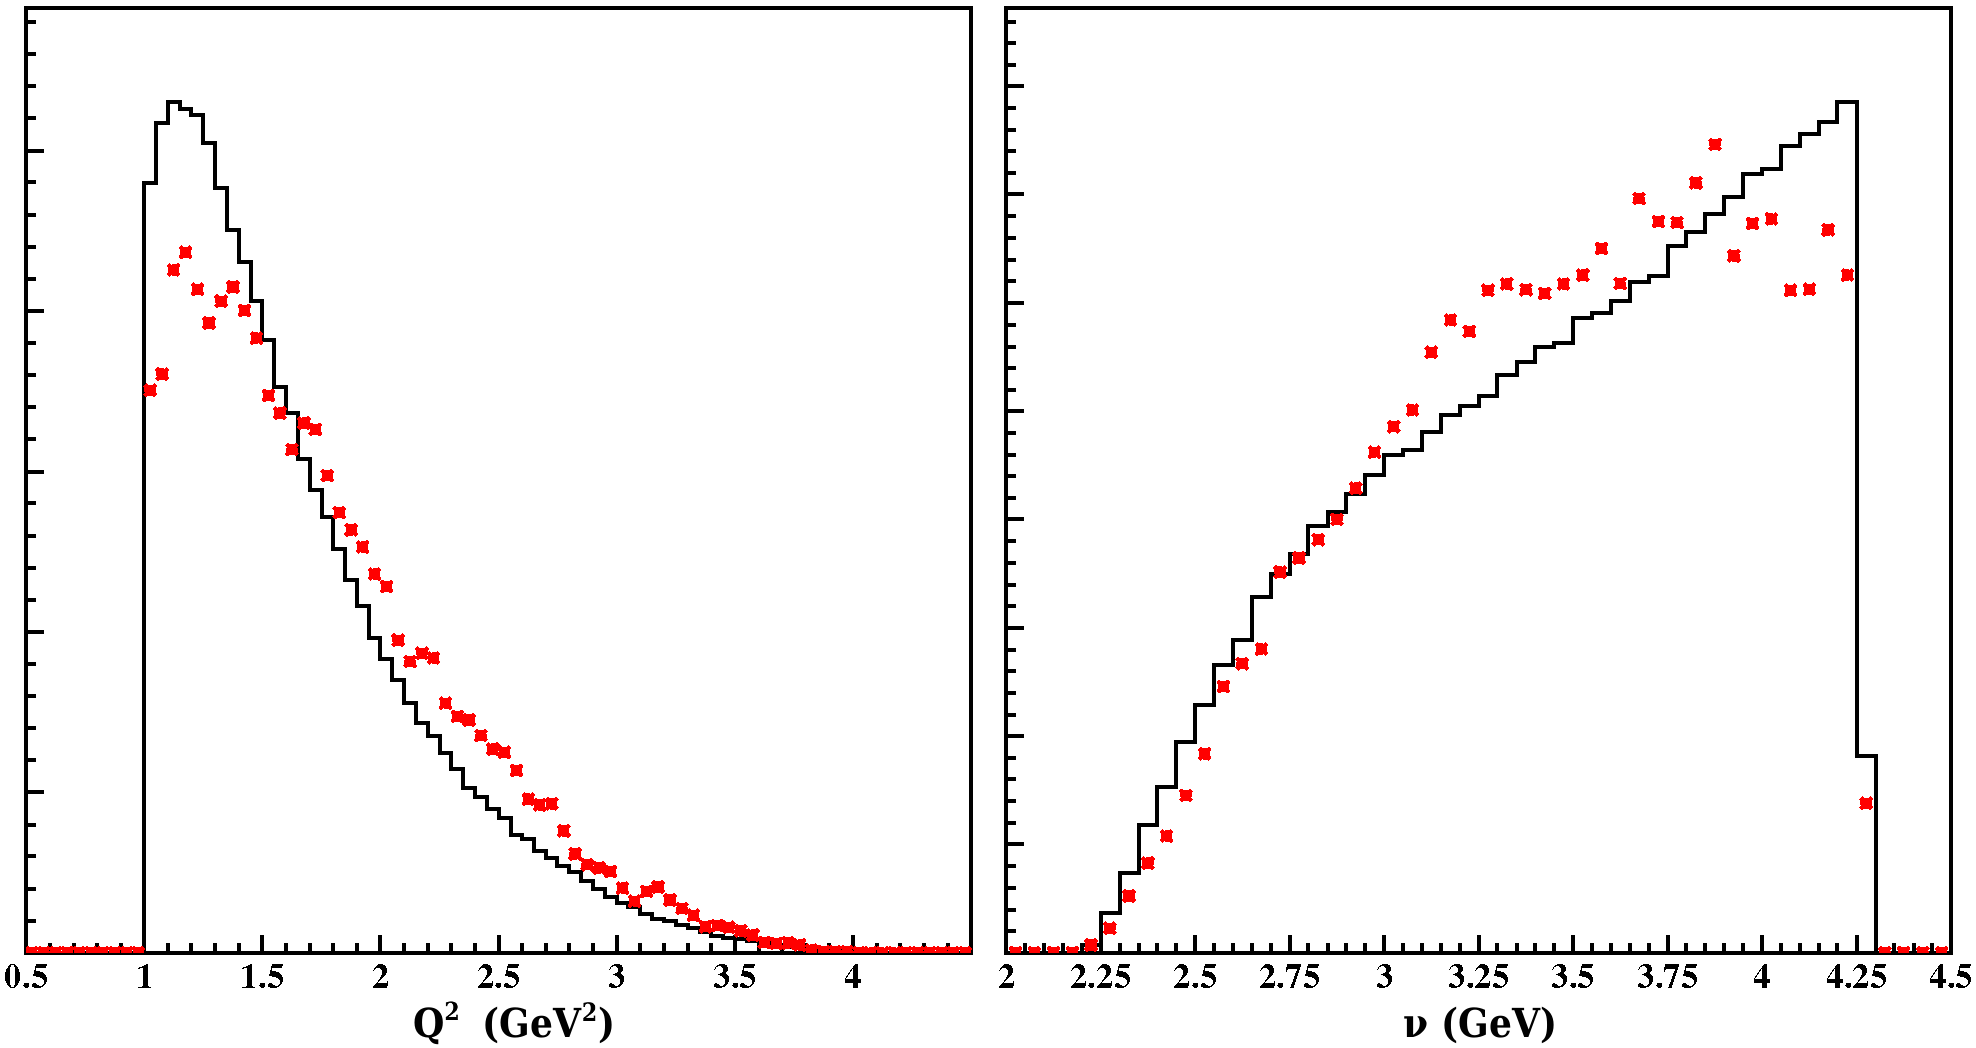
\includegraphics[width=12cm] {chap5-fig/El_compar.png}
\caption {Comparisons, for $Q^2$ (GeV$^2$/c$^2$) and $\nu$ (GeV), of the distributions
from simulated (red crosses) and experimental (histogram) data using deuterium target.}
\label{fig:compNuQ2}
\end{figure}

\begin{figure}[tbp]
\centering
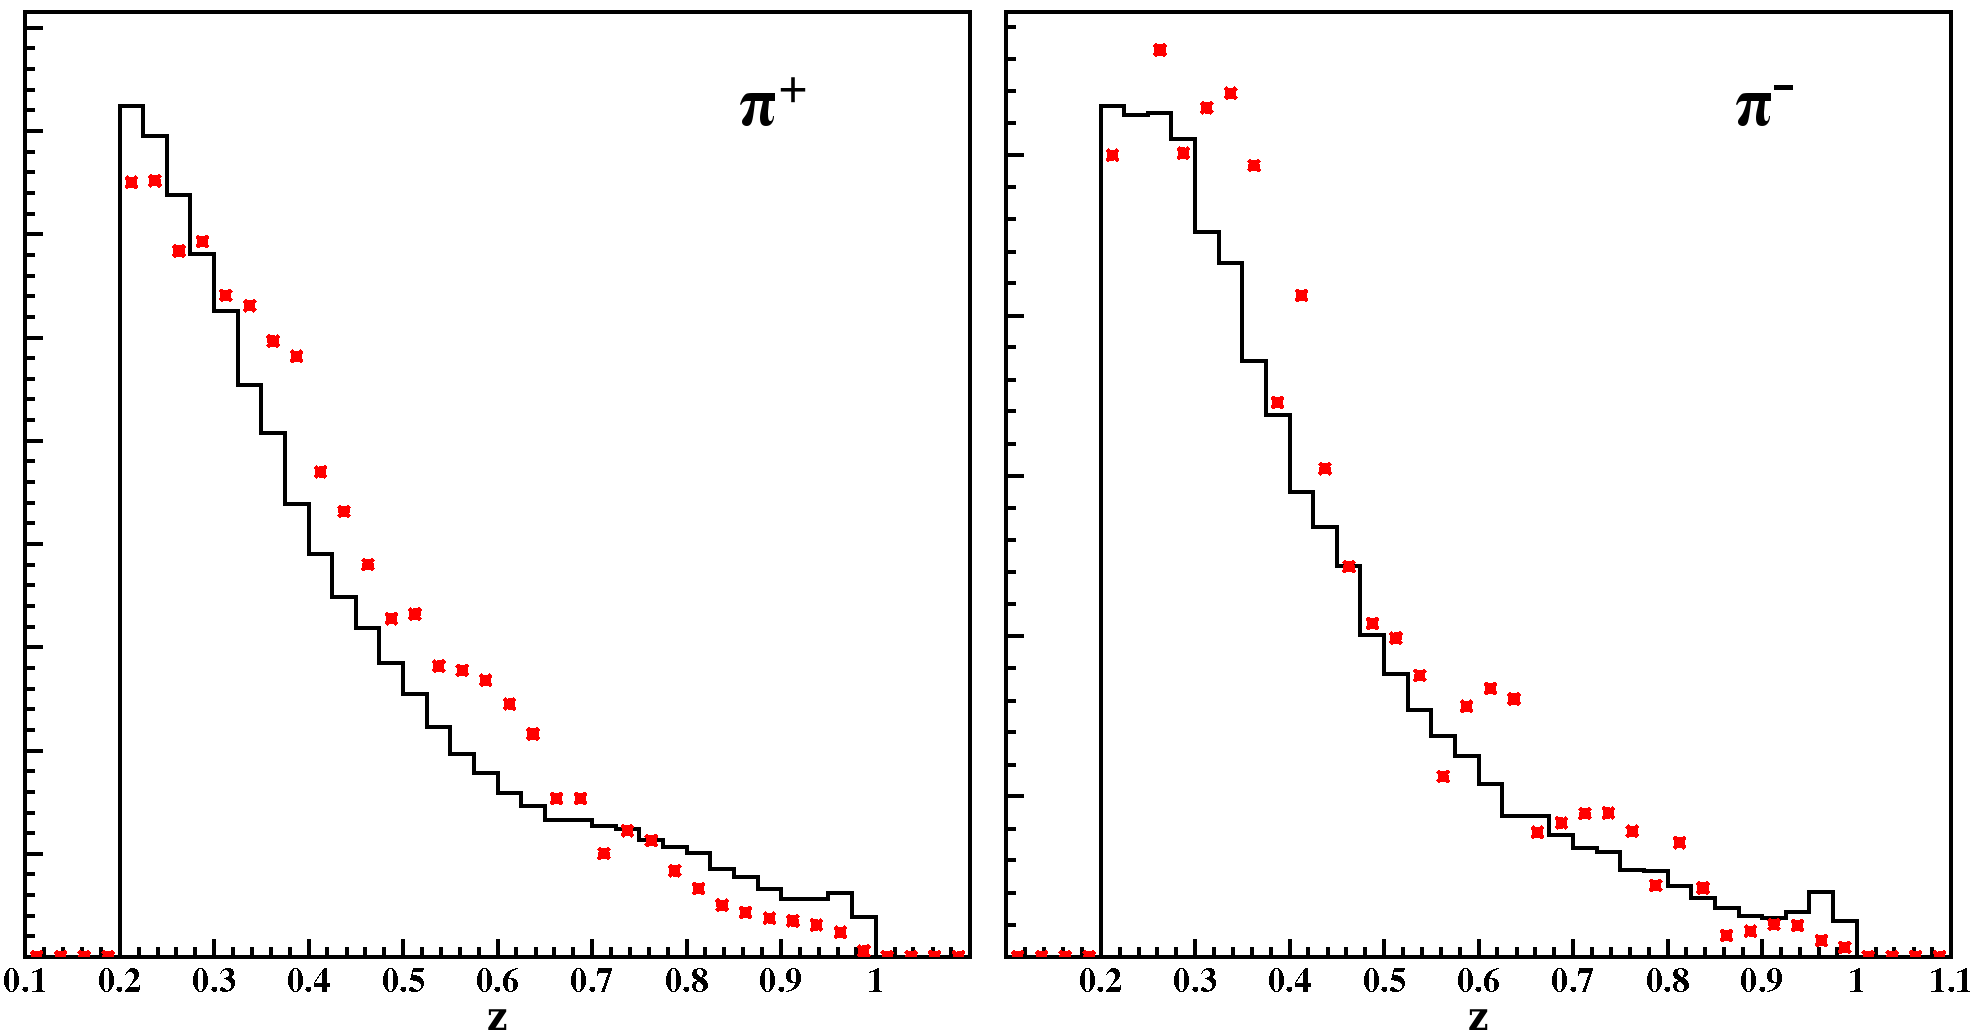
\includegraphics[width=12cm] {chap5-fig/z_compar.png}
\caption {Comparisons, for $z$ of charged pions, of the distributions
from simulated (red crosses) and experimental (histogram) data using deuterium target.}
\label{fig:compZ}
\end{figure}

\begin{figure}[tbp]
\centering
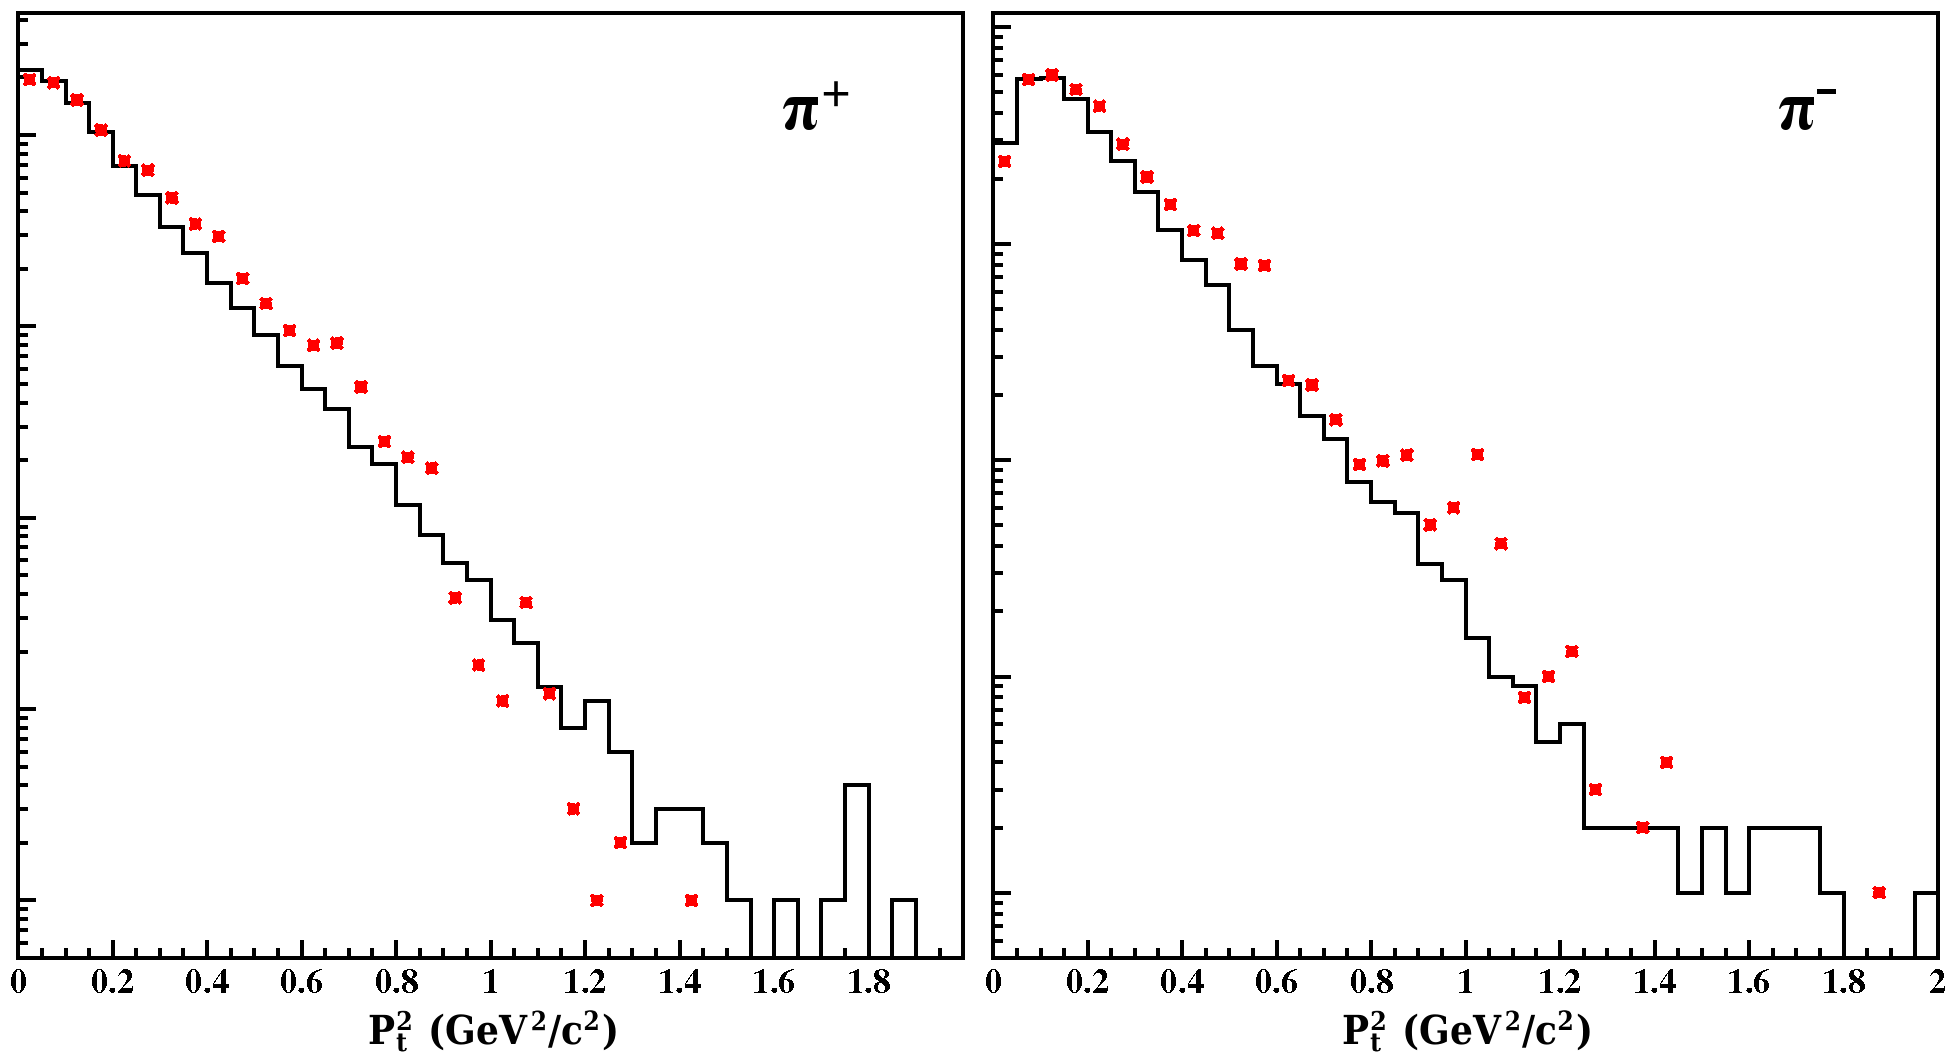
\includegraphics[width=12cm] {chap5-fig/pts_compar.png}
\caption {Comparisons, for \pt (GeV$^2$/c$^2$) of charged pions, of the distributions
from simulated (red crosses) and experimental (histogram) data using deuterium target.}
\label{fig:compPts}
\end{figure}

\begin{figure}[tbp]
\centering
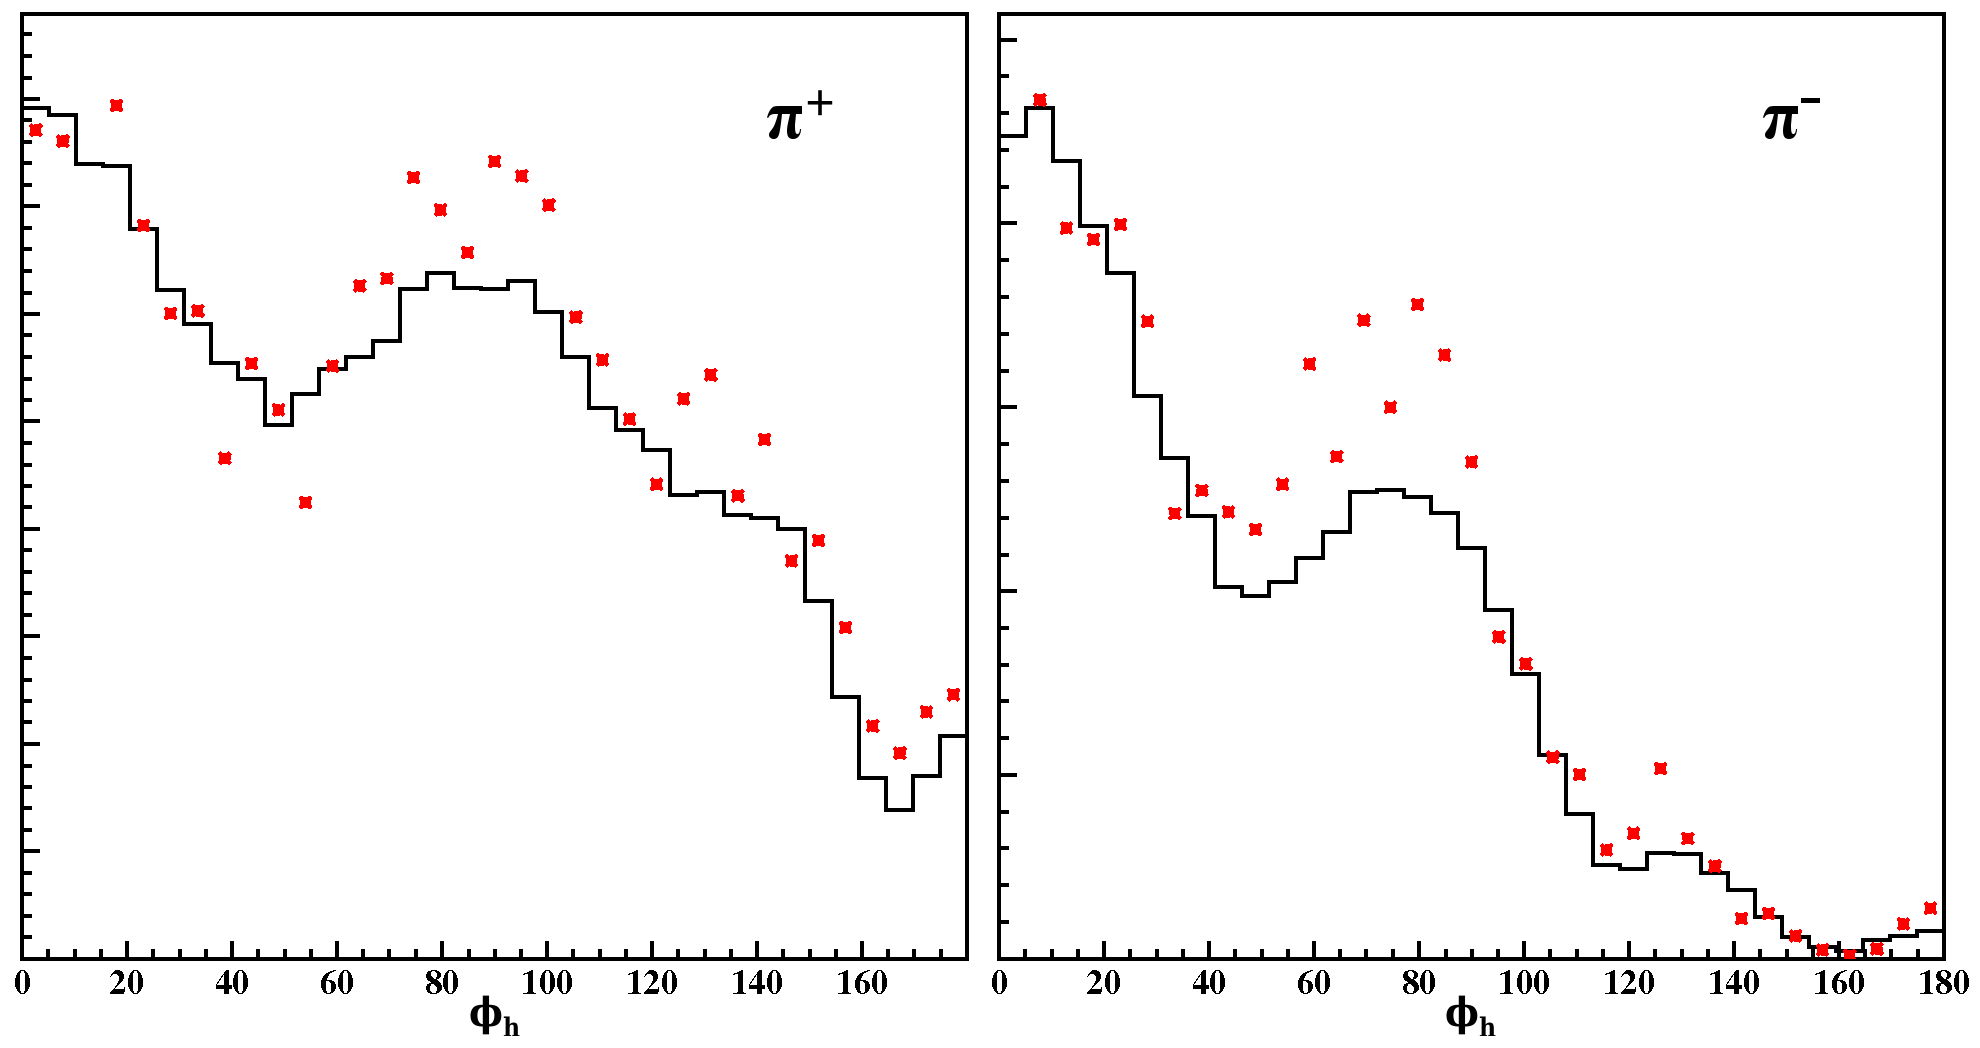
\includegraphics[width=12cm] {chap5-fig/phih_compar.png}
\caption {Comparisons, for $\phi_h$ of charged pions, of the distributions
from simulated (red crosses) and experimental (histogram) data using deuterium target.}
\label{fig:compPhih}
\end{figure}


\paragraph{Correction of the Data}

The acceptance correction coefficients are defined as the ratio of reconstructed and generated events,

\begin{equation}
\label{eq:acc}
\text{Acc} = {N_{rec} \over N_{gen}}.
\end{equation}

Experimental data were corrected using the weights defined as $\omega = 1/\text{Acc}$. These coefficients are calculated in many bins, in order to be independent of the imperfections of our event generator. However, an excess of bins could lead to a strong bin migration\footnote{Fraction of events not reconstructed in the bin they were produced in.}, which might introduce a bias in case it becomes quite large.

We used a 4-dimensional binning to divide the large phase space of our two particles' final state. However, to evaluate the associated systematic errors with this correction, we used the two different binning presented in table~\ref{tab:AcceptBinning}. The total number of bins is constrained by the amount of generated data, and must be maintained reasonably low in order to keep a good statistical precision and a manageable bin migration.

\begin{table}[htbp]
  \centering
  \begin{tabular}{@{} cc @{}}
    \hline
    Variable & Number of bins \\ 
    \hline
    $\nu$    & 5 \\
    $x_{Bj}$ & 5 \\
    $p_h$    & 7 \\
    $t$      & 7 \\
    \hline
    Total    & 1225 \\
    \hline
  \end{tabular}
  \begin{tabular}{@{} c @{}}
  ~~~~~~\\
  ~~~~~~\\
  \end{tabular}
  \begin{tabular}{@{} cc @{}}
    \hline
    Variable & Number of bins \\ 
    \hline
    $Q^2$    & 5 \\
    $\nu$    & 5 \\
    $z_h$    & 7 \\
    $t$      & 7 \\
    \hline
    Total    & 1225 \\
    \hline
  \end{tabular}
  \caption{Variables and their associated number of bins used on the 
   multi-dimensional binning of our acceptance correction. The left panel 
   shows the variables used on this correction, and the right panel contains the 
   variables used on the evaluation of the related systematic uncertainties.}
  \label{tab:AcceptBinning}
\end{table}

The weights ($\omega_{\pi^\pm}(\nu,x_{Bj},p_h,t)$) are then extracted from 
the simulation using equation \ref{eq:acc}. However, it turned out that these coefficients should not be applied to data before resolving the issue of the problematic bins that have either
\begin{itemize}
 \item too large weight values, i.e., very small acceptance, or
 \item very few reconstructed events leading to large statistical errors, or
 \item a large fraction of events originally generated in an other bin (bin migration issue).
\end{itemize}
To eliminate these bins we apply the following cuts:
\begin{equation} \label{eq:AccL1}
\left ({\delta \omega \over \omega}\right ) ^2 \times R_c \times \omega < 2,
\end{equation}
and
\begin{equation} \label{eq:AccL2}
N_{rec} > 4,
\end{equation}
where $\delta \omega / \omega$ is the relative error on the weight, and $R_c$ is the 
proportion of reconstructed events initially generated in an other kinematical bin. Figure \ref{fig:AccCoef} shows $\omega$ distributions after applying these cuts. Around 900 bins remain for both targets, but we noticed that these weights are much larger for $\pi^-$ compared to $\pi^+$, as an indication of a larger correction for the inbent particles. In order to maximize the acceptance and reduce the sensitivity to our arbitrary weights' cuts, we corrected the data with an additional two dimensional reweighting factor as:
\begin{equation}
\text{Acc}_2(\nu,p_h) = {\sum_{rec} \omega (\nu,x_{Bj},p_h,t)\over N_{gen}(\nu,p_h)}.
\end{equation}
where $\omega$ is the previously calculated weight of either one remaining bin or a bin that was excluded by the cuts. One of the criteria for setting the limits in equation \ref{eq:AccL1} and 
\ref{eq:AccL2} is to keep reweighting factors, $\omega_2 = 1/\text{Acc}_2$, at the level of a few percents.

\begin{figure}[tbp]
\centering
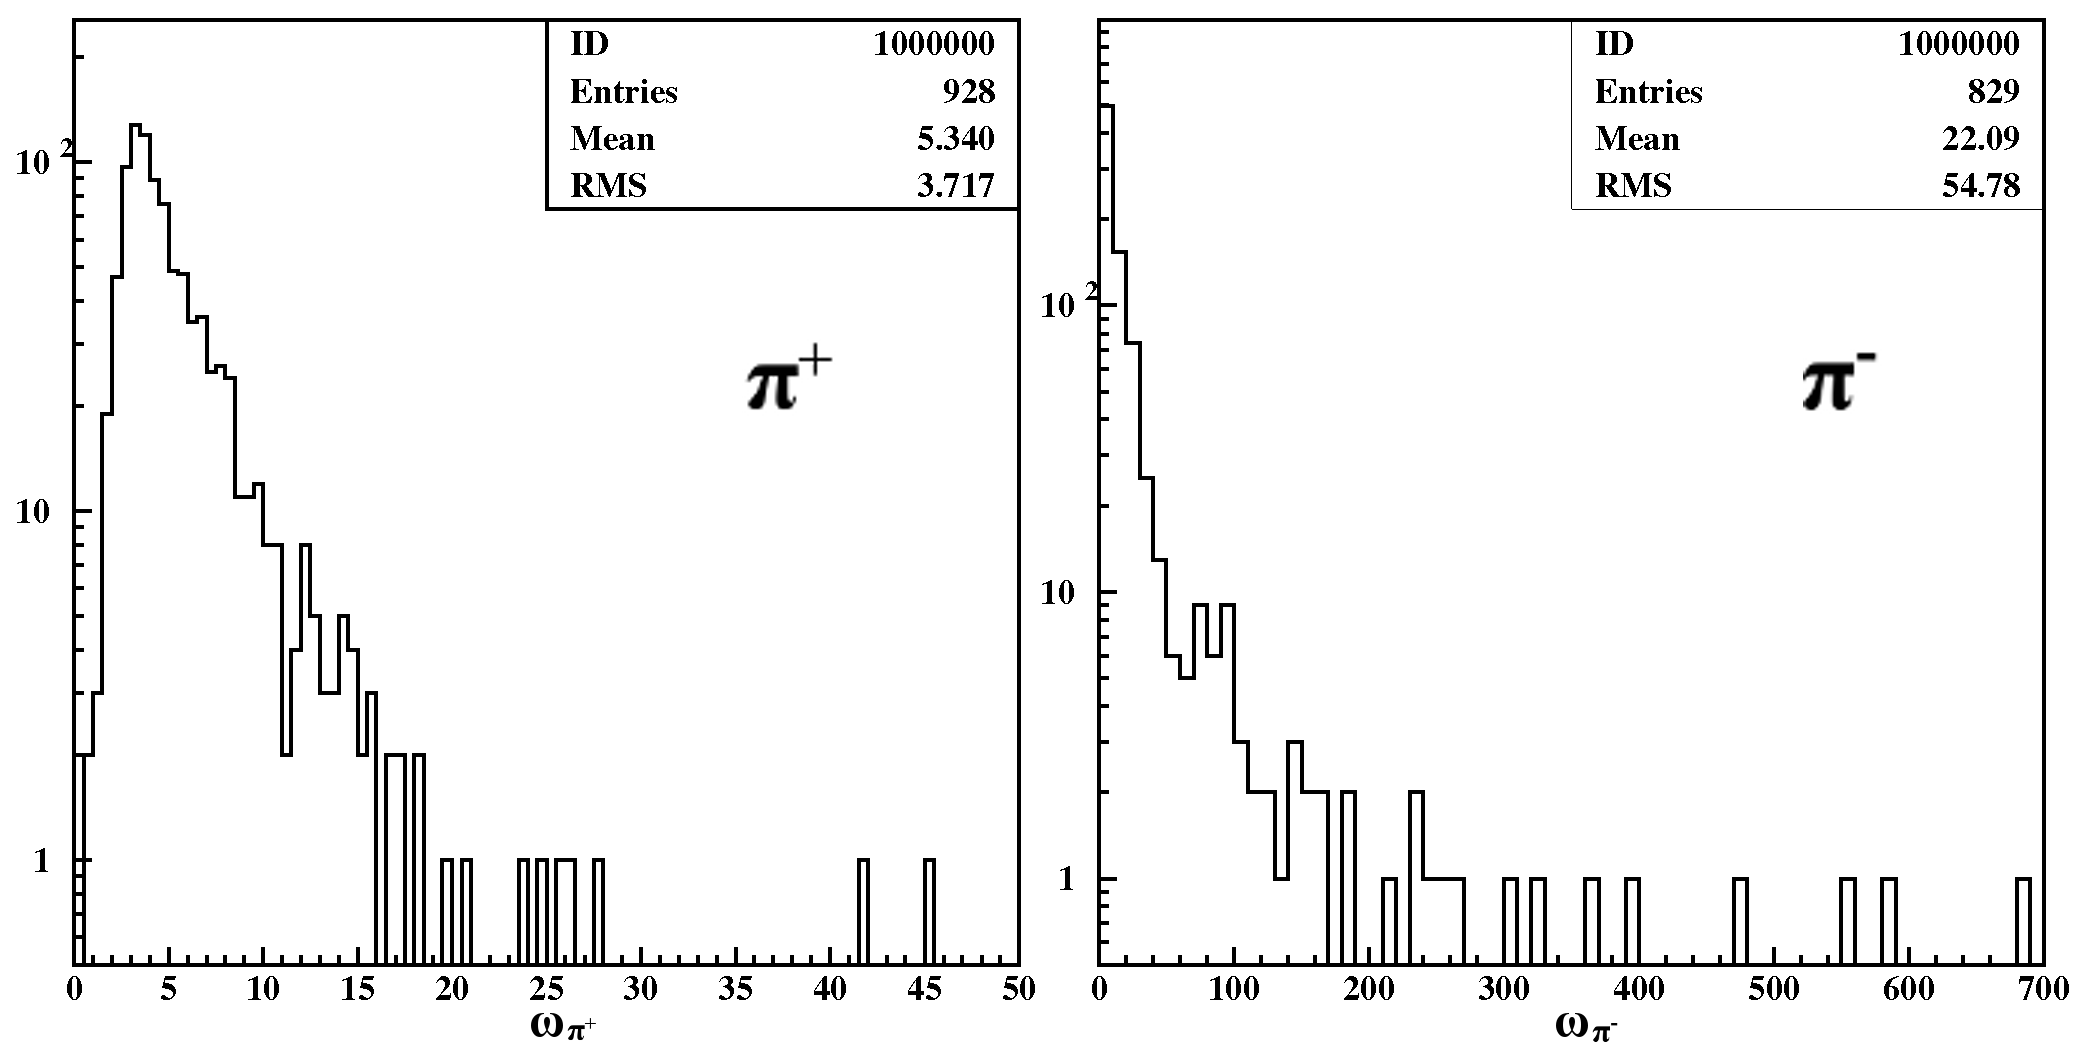
\includegraphics[width=14cm] {chap5-fig/pawpipdeut.png}
\caption {The extracted acceptance correction weights for pions on a deuterium target (not re-weighted).}
\label{fig:AccCoef}
\end{figure}

In order to correct the number of electrons in multiplicity ratios, we followed the semi-inclusive acceptance correction method by using only the two first dimensions ($\nu$ and $Q^2$). However, the reweighting was not used for electrons as all non-empty bins pass the two cuts, \ref{eq:AccL1} and \ref{eq:AccL2}.

\begin{figure}[tbp]
\centering
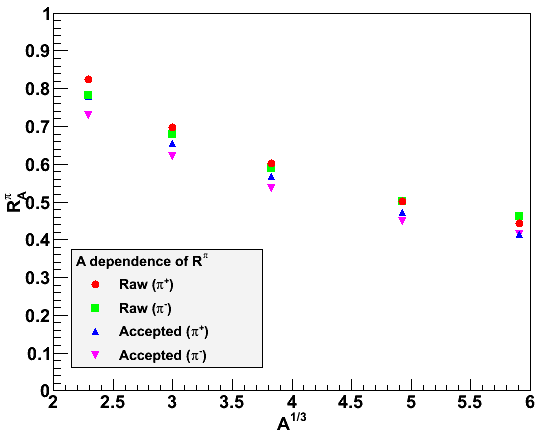
\includegraphics[width=7.4cm] {chap5-fig/b_RvA.png} 
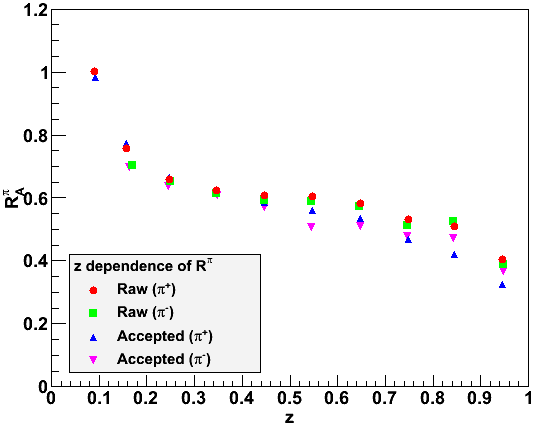
\includegraphics[width=7.4cm] {chap5-fig/b_RvZ.png} 
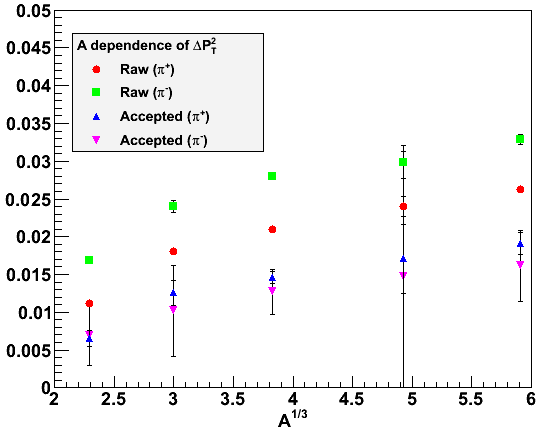
\includegraphics[width=7.4cm] {chap5-fig/b_PvA.png} 
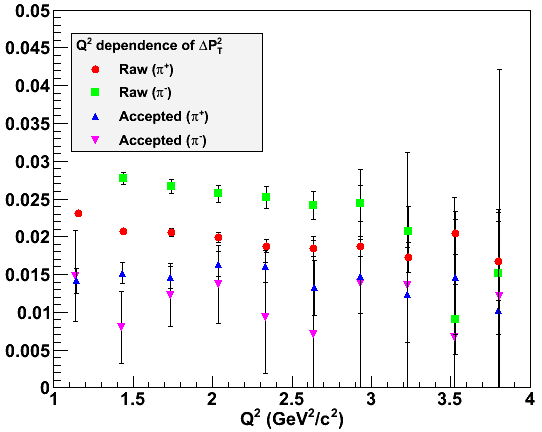
\includegraphics[width=7.4cm] {chap5-fig/b_PvQ2.png} 
\caption {Preliminary results are compared with the acceptance corrected ones, 
for multiplicity ratios (top) and transverse momentum broadening 
(bottom). Only statistical errors are shown.}
\label{fig:AcceptPlots}
\end{figure}

Figure \ref{fig:AcceptPlots}, where only statistical errors are 
represented, shows the new results after applying the acceptance correction.
The acceptance correction effects appear to be in the order of $10$\% for 
multiplicity ratios and $30$\% for the transverse momentum broadening. This is a surprisingly significant correction with regard to a few centimeters separating the two targets. The reason for such a large correction is that the small shift in the $z$-vertex position changes slightly the minimum angle of the detector in the region where most hadron production is concentrated, {\it i.e.} at low \pt close to the beam line. The $\pi^-$s were more affected due to the inbending magnetic field. Indeed, the low \pt $\pi^-$s had very low acceptance which led to large correction factors. The large spread in weights makes the errors on \dpt very large, and the related results difficult to exploit. However, our transverse momentum broadening results of both pions matched each other after this correction, which is consistent 
with HERMES results.

\subsubsection{Coulomb Correction}
\label{CCor}

The large electric charge of our nuclear targets create an electric field that should be taken into account at our energies. Besides the fact that the nuclear electric field accelerates or decelerates the incoming and outgoing charged particles, it has some non trivial effects such as the focusing of low energy particles. Aste {\it et al.}~\cite{Aste:2005wc} showed that these Coulomb effects could be corrected for by using an effective momentum approximation at large momenta ({\it i.e.}, $Q^2>.5$ GeV$^2$). As our kinematics coverage is beyond this limit, we decided to use this approximation on the coulomb correction of our data-sets. According to Aste {\it et al.}, the best effective potential approximation is given by $\bar V= 0.8 V_0$, where $V_0$ is the electrostatic potential at the center of nuclei. The latter is evaluated as $V_0= -3 \alpha_{EM} Z / (2 R)$, where $\alpha_{EM}$ is the fine-structure constant, Z is the proton number, and R is the radius of nuclei. Table 5 contains the used values of $V_0$ and $\bar V$ on different nuclear target's analysis. We must note that this Coulomb correction has been applied to both electrons and charged pions before calculating any kinematical variables.

\begin{table}[htbp]
  \centering
  \begin{tabular}{@{} ccc @{}}
    \hline
Nucleus & $V_0$ (MeV)  &  $\bar V$ (MeV) \\ \hline
$^2$H  & -1  &     -1 \\
C   &  -4 &      -3 \\
Al  &  -7 &      -6 \\
Fe  & -11 &    -9 \\
Sn  & -17 &   -14 \\
Pb  & -23 &   -19 \\
    \hline
  \end{tabular}
  \caption{The $V_0$ and $\bar V$ values used on Coulomb corrections for different charged particles.}
  \label{tab:Coulomb}
\end{table}

\subsubsection{Radiative Correction}
\label{RadCor}

Despite its lower magnitude compared to the strong force, the 
electromagnetic force may have a non negligible impact on our results. The 
reason is that even a moderate energy photon emission can modify significantly the measured kinematical variables. To correct this effect, several simulation codes exist \cite{Akushevich:2001yp}, however, none of them treat directly the SIDIS production on nuclei. For that reason, a dedicated Monte-Carlo simulation based on existing codes was developed.

\paragraph{Simulation}

The inclusive radiative effects are generated using the RADGEN code 
\cite{Akushevich:1998ft}, which includes Feynman diagrams shown in 
figure~\ref{fig:FDRadCorr}. Using this code one can evaluate the correction 
factors for inclusive measurements as $\delta = \sigma_{obs} / \sigma_{Born}$, where $\sigma_{obs}$ is the measured inclusive cross section, and $\sigma_{Born}$ is the Born cross section. As RADGEN is also a Monte-Carlo generator for photon emissions, it could be used to modify the virtual photon kinematics before the 
hadron production in any DIS generator. This allows the evaluation of the radiative 
effects on semi-inclusive measurements by implementing RADGEN inside the main 
Monte-Carlo event generator.

\begin{figure}[htp]
\centering
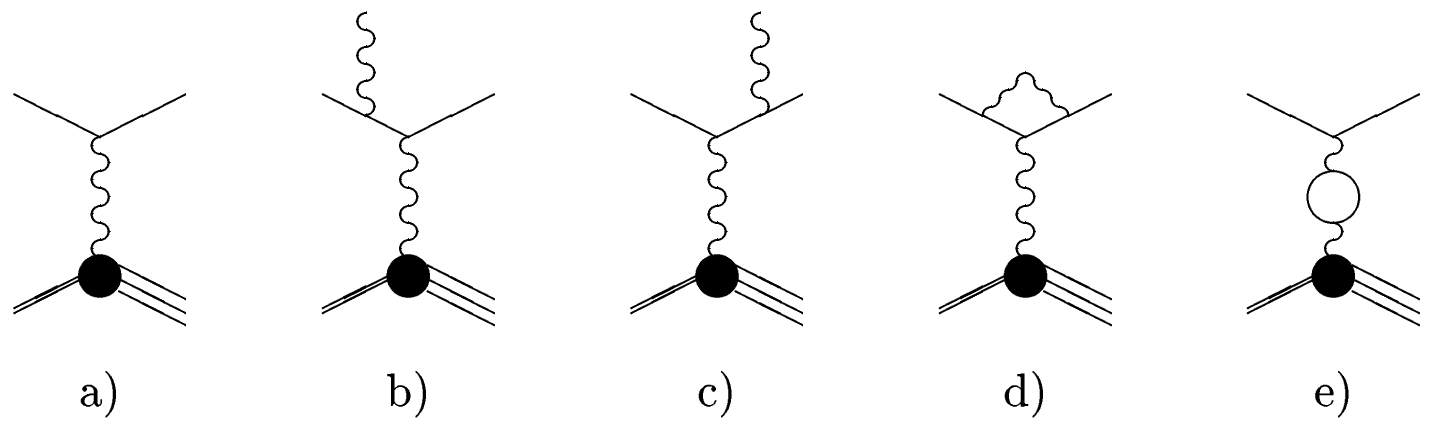
\includegraphics[width=12cm] {chap5-fig/RadDiag.png}
\caption {Diagrams taken into account in RADGEN \cite{Akushevich:1998ft}. The 
diagrams b) to e) contribute to the first order calculation of the radiative 
effects on Born cross section (diagram a)).}
\label{fig:FDRadCorr}
\end{figure}

The Monte-Carlo simulation was done using the event generator, GENIE~\cite{Andreopoulos:2009rq}, that describes well electron-nucleus interactions. Indeed, GENIE contains the quasi-elastic scattering\footnote{Elastic 
scattering off a single nucleon on nuclei.}, which is considered as the main channel generating radiative events in the DIS region \cite{Akushevich:2007jc}. This generator includes also hadronic cascades in nuclei, at which pions might be generated in quasi-elastic events. This is an important feature because the quasi-elastic production can not contribute directly to semi-inclusive measurements.

\paragraph{Correction of the Data}

We generated 100 million events with and without radiative effects for each target. The RADGEN code gave us the magnitude of inclusive correction coefficients, however, the comparison between the two data sets allows the extraction of semi-inclusive correction factors.

The ratio of inclusive correction factors, as depicted in figure \ref{fig:RadCorrFac}, is relatively small (couple of percents at most) except for low \xb and high $\nu$. Similarly for the semi-inclusive factors' ratio shown in figure \ref{fig:RadCorrFacSIDIS} as a function of $z$ and \ptp. However, the associated statistical errors are quite large because only a small fraction of the events involved a photon radiation.

\begin{figure}[htbp]
\centering
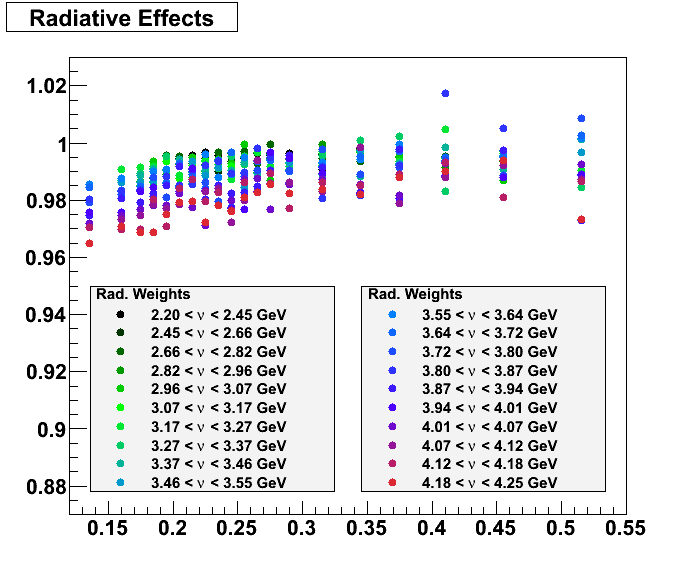
\includegraphics[width=9cm] {chap5-fig/ElecRadWei_Lead.png}
\caption {Ratios of radiative correction factors, $\delta_\text{Pb}/
\delta_{^2\text{H}}$, as a function of \xb in various $\nu$ bins.}
\label{fig:RadCorrFac}
\end{figure}

\begin{figure}[htbp]
\centering
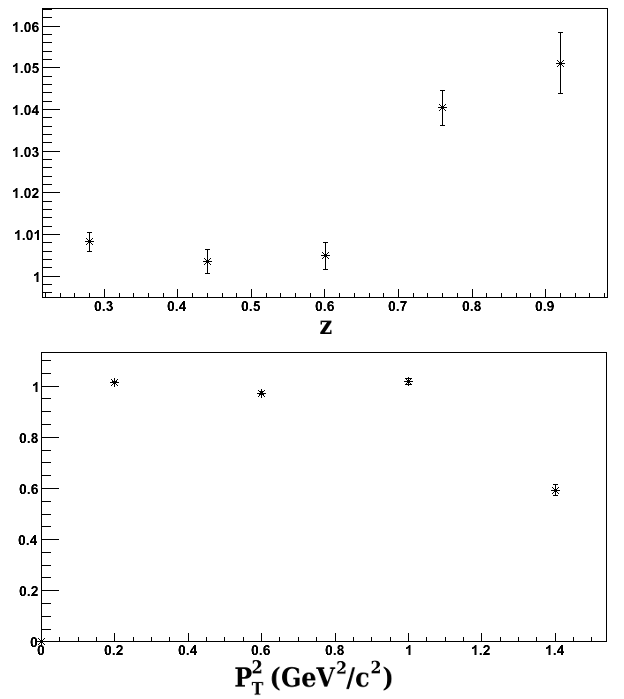
\includegraphics[width=9cm] {chap5-fig/RadGenFactors.png}
\caption {Ratios of radiative correction factors, $\delta_\text{Pb}/
\delta_{^2\text{H}}$, as a function of $z$ (top) and \ptp (bottom).}
\label{fig:RadCorrFacSIDIS}
\end{figure}

The semi-inclusive part of the radiative correction turned out to be limited 
in amplitude for the most kinematics, except for high $z$ and \ptp. Thus, we decided to not apply this correction before further studies.

{\color{red} We found a better way to implement the radiative correction,
that is not limited by the used MC technique. We will implement it in
the second version of the note as we do not want to delay the review process because this correction that we already found to be small. Sorry about that.}

\subsubsection{Isospin Correction}

The important excess of neutrons in heavy nuclei leads to a modification of both $\pi$ multiplicities on DIS events. Using Hall~C results 
\cite{Asaturyan:2011mq}, shown in figure \ref{fig:IsoSpin}, we evaluated the correction factors for this effect. Our simple estimation is solely based on 
proton and neutron numbers that gave $\pi^+$s results shown in table~\ref{tab:isospin}. As the effect on $\pi^-$s was found to be consistent with zero, no correction was applied to their multiplicity ratios. 
We attribute a 10\% normalization error to the effect of the isospin correction on our results. It is relatively chosen based on the precision of the Hall~C measurement, and the limited phase space coverage of Hall-C data compared to ours.

\begin{figure}[tbp]
\centering
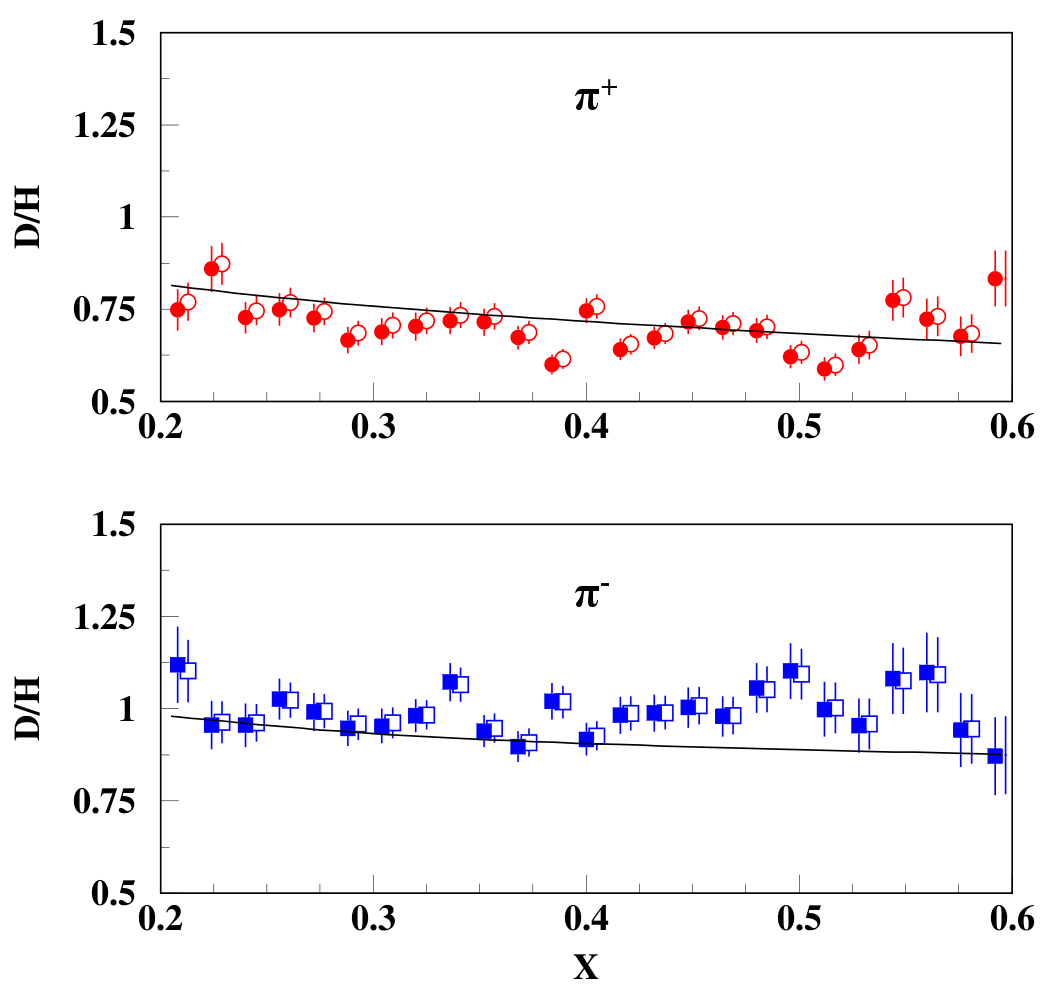
\includegraphics[width=10cm] {chap5-fig/HallC-Isospin.png}
\caption {Ratios of deuteron over proton for $\pi^+$s (top) and $\pi^-$s (bottom)
as a function of \xb at $z=0.55$ \cite{Asaturyan:2011mq}.}
\label{fig:IsoSpin}
\end{figure}

\begin{table}[htbp]
  \centering
  \begin{tabular}{@{} cc @{}}
    \hline
    Target & Isospin  \\ 
           & correction \\ 
    \hline
    C & 0 \\
    Al & 1.5\%\\
    Fe &  3\% \\
    Sn &  8\%\\
    Pb &  10\% \\
    \hline
  \end{tabular}
  \caption{Isospin correction applied to $\pi^+$ multiplicity ratios for different targets.}
  \label{tab:isospin}
\end{table}

It is important to mention that the isospin correction is applied only to rates, which means applied only to $\pi^+$s multiplicity ratios. The transverse momentum broadening could, in principle, be affected, however, the results from \cite{Asaturyan:2011mq} showed no isospin effects in \ptp. Therefore, we are confident that our \dpt results should not be sensitive to any isospin effects.

We finally note that the $A$ dependence of multiplicity ratios of both charged pions became parallel after the isospin correction\footnote{Within 
normalization errors presented in section \ref{sec:TotSys}} (see figure 
\ref{fig:IsoPlot}). Considering previous measurements and existing models, 
this result was expected and demonstrated the importance of this correction.

\begin{figure}[tbp]
\centering
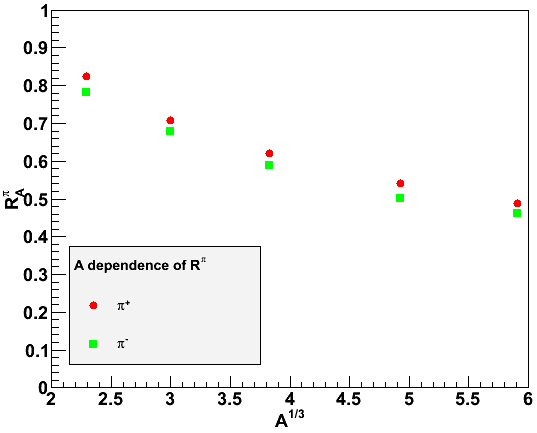
\includegraphics[width=8cm] {chap5-fig/c_RvA.png}
\caption {Multiplicity ratios as a function of $A^{1/3}$ 
with only the isospin correction applied.}
\label{fig:IsoPlot}
\end{figure}

\subsection{Systematic Uncertainties}
\label{sec:TotSys}

In this section, we are presenting details of our two types of systematic uncertainties. The point-to-point systematic errors, that vary with kinematical variables, were calculated bin by bin for each result. They are caused by uncertainties on the particles' identification cuts and the CLAS acceptance. The normalization errors are attributed globally since they don't depend on kinematics. They are due to acceptance effects, target's misidentification, and the isospin correction.

\subsubsection{Quality of the Detection}
\label{SysId}

The simulation of the CLAS detector, using the GSIM package, is used 
to evaluate the systematic errors correlated with:

  - experimental resolution of kinematical variables,

  - particles' misidentification,

  - particles' re-scattering in different detectors,

  - particles' energy loss.\\


To evaluate those errors, we are comparing the kinematics of reconstructed particles with the generated ones. Each reconstructed particle is associated with its generated parent if both particles have a similar momentum and angle coverage. However, the precision of the measured kinematical distribution $\Delta p$, $\Delta \theta$ and $\Delta \phi$ were determined as $\Delta x = {\sum_n |x_{gen} - x_{rec}| \over n}$, where $n$ is the kinematical bin number. Using the same simulation as for the acceptance, we found ${\delta p \over p } = 0.03$, $\delta \theta = 3$ mrad and $\delta \phi = 10$~mrad. Nevertheless of being much larger than the nominal CLAS resolutions published in \cite{Mecking:2003zu}, they are still reasonable for our measurement. Although, we evaluated the systematic errors associated with other variables\footnote{These values were evaluated for a typical kinematics range. However, the results can be much larger at extreme kinematics (large \pt or Q$^2$).}, such as $\delta Q^2 \sim 0.013$ GeV$^2$/c$^2$, $\delta z \sim 0.4 \%$, and $\delta P_\perp^2 \sim 0.004$ GeV$^2$/c$^2$. These errors are overall negligible since they are several times smaller than our usual bin sizes (see figures in a section \ref{prelim}). 

We also evaluated the particles' misidentification and the re-scattering effect in different detectors or coils. The misidentification usually leads to a high 
contamination on the kinematical distributions tails, which is manifested most in our case on the tail of the \pt distribution. This effect is due to a low probability to produce high \pt events, therefore the contribution from the accidental background is relatively increased. As a consequence, we used the following cut $p_\perp^2 < 2.5$~GeV$^2$/c$^2$, which basically discarded only a very little amount of data (about one $\pi$ from 30000 pions). The misidentification of electrons was found to be too small in the order of $1\,e^-$ each 1000 events, hence does not contribute significantly to this uncertainty. For pions, the main contamination comes from kaons with momenta above 2~GeV/c ($\sim$ 3\% for $\pi^+$s and $\sim$ 0.5\% for $\pi^-$s). Protons also contaminates a $\pi^+$ sample at high momenta (up to a few \%). 
%TODO Justify the pt cut with a figure?

In conclusion, the uncertainty related to particles' misidentification is taken into account in the point-to-point systematic errors by assuming a 100\% contamination level. Other effects were found negligible.

\subsubsection{Target Reconstruction}

Because of some reconstruction errors or a re-scattering on detectors' materials, it 
is possible to associate a particle with the wrong target. To estimate this 
effect, we looked, in the experimental data, at the number of reconstructed events upstream and downstream our targets, where nothing should be detected. Thus, we defined two test regions (see figure \ref{fig:targetleak}) to evaluate a targets' contamination. The upstream region, named as a test region 1, was given the size of the solid target's selection cut to evaluate the contamination from the liquid target. However, the downstream region, named as a test region 2, covered the same size of the liquid target's selection cut to estimate the leak from the solid target. The distance between detection and test regions is identical to the 
distance between the two targets' detection regions. 

We found that the number of electrons in the test region 1 and 2 represents, 
respectively, 1 and 2\% of the total number of events. However, in the case of semi-inclusive measurements, where we request two particles in the final state, this number drastically dropped, and became in the order of 0.01\%. In conclusion, only the number of electrons is significantly affected by a target's contamination issue, which leads to a normalization error of 1\% in all multiplicity ratios.

\begin{figure}[tbp]
\centering
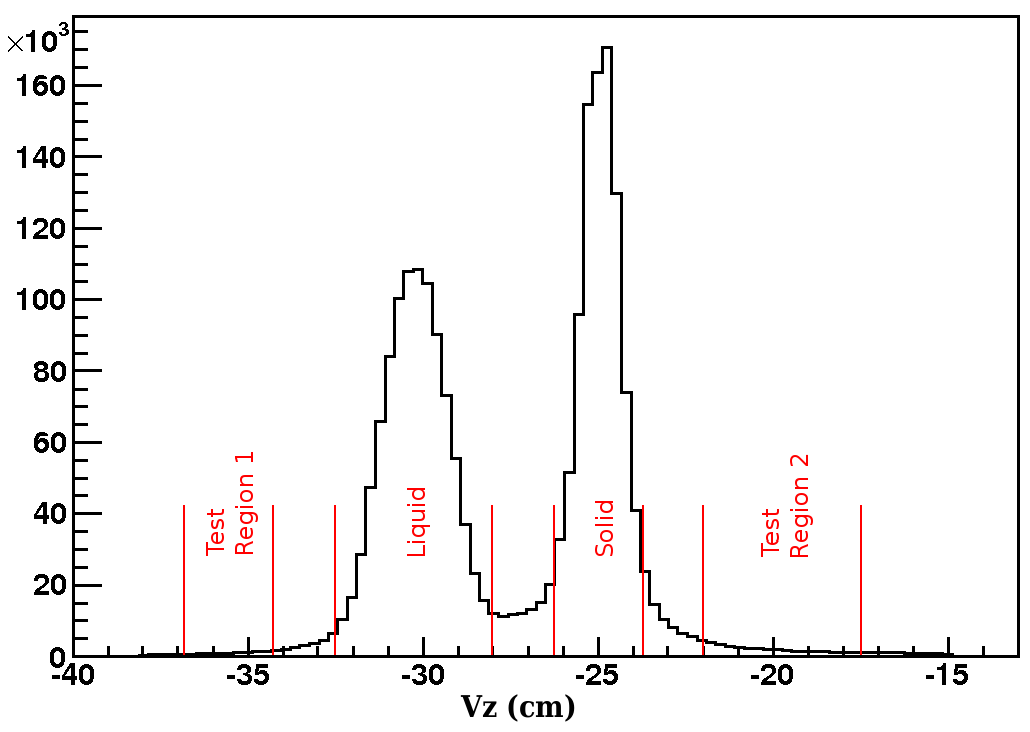
\includegraphics[width=9cm] {chap5-fig/Vertex.png}
\caption {Vertex distribution along a z direction (in cm), i.e. along the 
beam line. In red are shown the cuts used to evaluate the leak from one target to 
another.}
\label{fig:targetleak}
\end{figure}

\subsubsection{Acceptance}

After testing several different acceptance correction methods, we finally converged with the one using the two different binning presented on a table \ref{tab:AcceptBinning}. The difference between these methods gave us an idea about the systematic error associated with this correction. Using our results on iron, we found the relative uncertainties presented in a table~\ref{tab:SysAcc}. We noticed the significantly large errors for $\pi^-$s, which were expected, due to their low acceptance and larger weights. Although, systematical errors are considerably large on \dpt measurements. This is mainly due to the nature of the \dpt observable; as a difference, it would indeed enhance relative errors significantly. As it was shown in figure~\ref{fig:AcceptPlots}, error bars became much larger for the corrected \dpt from the acceptance effect. This fact indicated an important statistical sensitivity introduced by our weighting methods. The errors on \dpt are of the same order, or smaller, than the differences observed between the two weighted data-sets. This is an indication that the uncertainties reported in table \ref{tab:SysAcc} are, in nature, similar to the statistical errors, in the sense that both originate from the large variation between event-by-event weights. For this reason, we decided to do not include this error in our systematic budget to avoid double counting this effect.

\begin{table}[htbp]
  \centering
\renewcommand{\arraystretch}{1.3}
  \begin{tabular}{|c|c|c|}
    \hline
    Variable & Normalization & Point to point \\ 
             & errors        & errors         \\ 
    \hline
    $R^{\pi^+}_A$  & 1.2\% & 1.5\%  \\
    $R^{\pi^-}_A$  & 2.5\% & 2.6\%   \\
    $\langle \Delta P_\perp^2 \rangle^{\pi^+}_A$ & 5\% & 11\% \\
    $\langle \Delta P_\perp^2 \rangle^{\pi^-}_A$ & 5\% & 21\% \\
    \hline
  \end{tabular}
  \caption{Relative errors on pions' observables using the two weighting methods described in the text.}
  \label{tab:SysAcc}
\end{table}

\subsubsection{Total Systematic Budget}

The point-to-point errors include contributions from a detection contamination and acceptance effects. However, the normalization errors, which are independent of kinematical variables and due to acceptance effects, a target's misidentification and the isospin correction, are summarized in a table~\ref{tab:sysid}. 

\begin{table}[htbp]
  \centering
\renewcommand{\arraystretch}{1.3}
  \begin{tabular}{|c|cc|cc|}
    \hline
              & $R_A^{\pi^+}$  & $R_A^{\pi^-}$ & \dptp$^{\pi^+}$ &  \dptp$^{\pi^-}$\\ 
    \hline
    Acceptance & 1.2\% & 2.5\% & 5\% & 5\% \\
    Target id. & 1\% & 1\% & 1\% & 1\% \\
    Isospin (Pb)& 1\% & 1\% & 1\% & 1\% \\
    Total      & 1.9\% & 2.9\% & 5.2\% & 5.2\% \\
    \hline
  \end{tabular}
  \caption{Total normalization uncertainties for both charged pions.}
  \label{tab:sysid}
\end{table}

